% !TeX document-id = {0beb03b8-2a83-45f5-aca6-99def446a6e3}
% !TEX TS-program = pdflatexmk
\documentclass[12pt]{article}
\usepackage{a4wide}
\usepackage{amsmath,amssymb}
\usepackage{bm}
\usepackage{enumitem}
\usepackage[colorlinks]{hyperref}
\usepackage{graphicx}
\usepackage{listings}
\usepackage{appendix}
\usepackage{color}
\usepackage{caption}
\newcommand{\vect}[1]{\hat{\boldsymbol{#1}}}
\usepackage{subcaption}
\usepackage{float}
\usepackage{multirow}

\usepackage{chngcntr}

\newcommand{\reporttitle}{Project Report : Data assimilation for the Lorenz system}
\newcommand{\reportauthorOne}{Melissa Aydogdu}
\newcommand{\reportauthorTwo}{Frédérique Lecourtier}
\newcommand{\reportsupervisorOne}{Christophe Prudhomme}
\newcommand{\reportsupervisorTwo}{Luca Berti}
\newcommand{\reporttype}{Coursework}

\hypersetup{
	colorlinks=true,
	linkcolor=blue,
	filecolor=magenta,      
	urlcolor=cyan,
	citecolor=cyan
}

% captions
\counterwithin{figure}{section}

\makeatletter
\usepackage[labelformat=simple]{subcaption}
\newcommand\captionsubfigure{%
	\renewcommand\p@subfigure{}
	\renewcommand\thesubfigure{\thefigure.\alph{subfigure}}
}
\makeatother

\begin{document}
	\nocite{*}
	
	\begin{titlepage}

\newcommand{\HRule}{\rule{\linewidth}{0.5mm}} % Defines a new command for the horizontal lines, change thickness here

\begin{center} % Center remainder of the page


\includegraphics[width = 0.5\linewidth]{images/logo-cemosis.pdf}\\[1.5cm] 

\textsc{\Large University of Strasbourg}\\[0.5cm] 
\textsc{\large Master CSMI}\\[0.95cm] 

%----------------------------------------------------------------------------------------
%	TITLE SECTION
%----------------------------------------------------------------------------------------

\HRule \\[0.4cm]
{ \huge \bfseries \reporttitle}\\ % Title of your document
\HRule \\[1.5cm]
\end{center}
%----------------------------------------------------------------------------------------
%	AUTHOR SECTION
%----------------------------------------------------------------------------------------

%\begin{minipage}{0.4\hsize}
\begin{flushleft} \large
	\begin{minipage}{0.4\hsize}
		\textit{Authors:}\\
		\reportauthorOne\\
		\reportauthorTwo
	\end{minipage} \hfill 
	\begin{minipage}{0.4\hsize}
		\textit{Supervisors:}\\
		\reportsupervisorOne\\
		\reportsupervisorTwo
	\end{minipage}
\end{flushleft}
\vspace{4cm}
\makeatletter
Date: \@date 

\vfill % Fill the rest of the page with whitespace



\makeatother


\end{titlepage}


	
	\tableofcontents
	
    \newpage
	\section{Roadmap}
	    \label{diag}
	    
	\begin{center}
		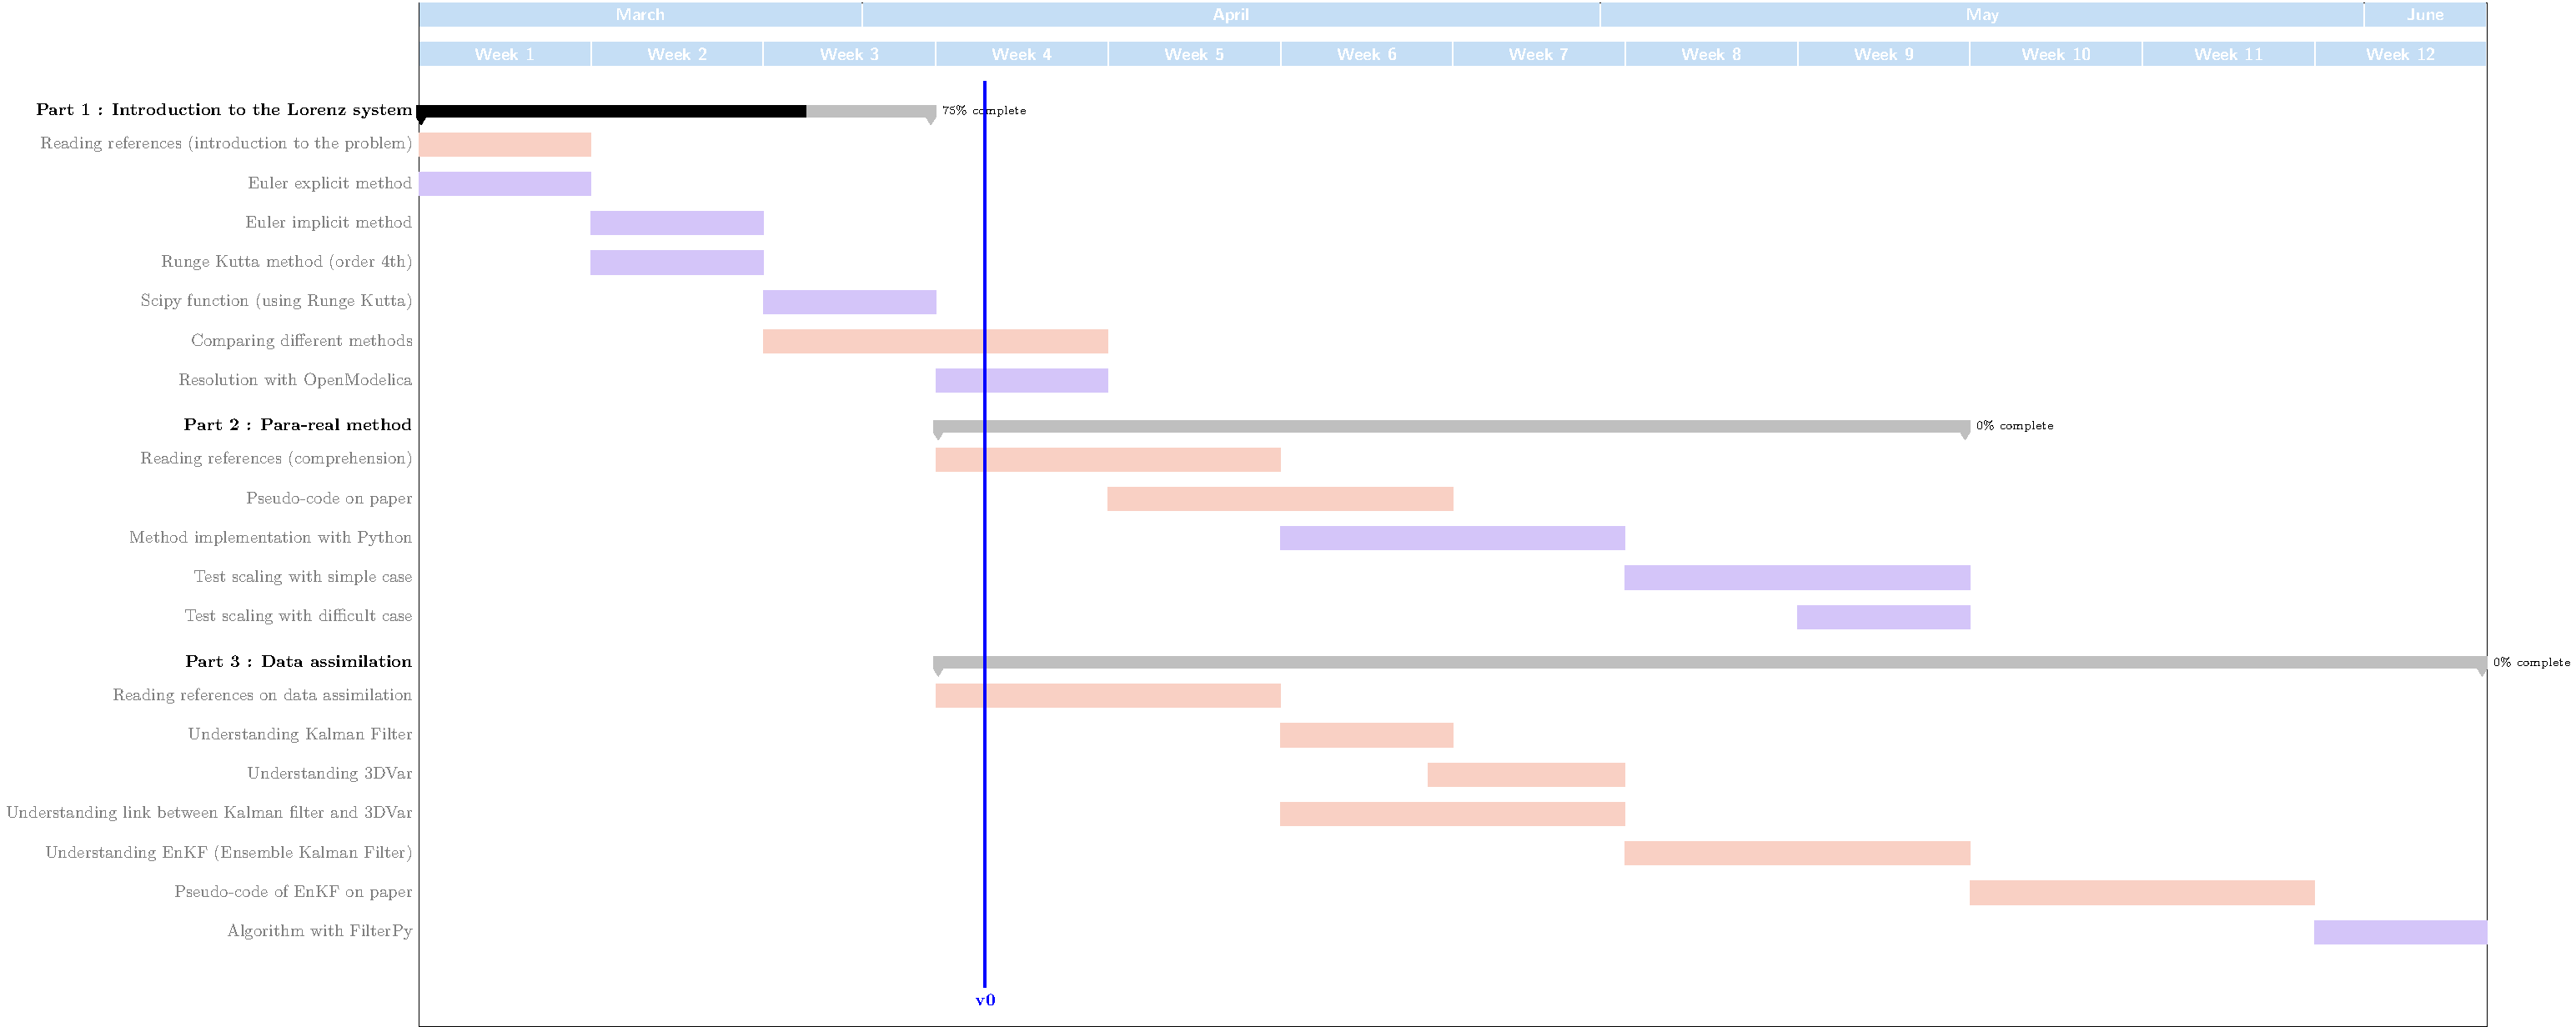
\includegraphics[angle=90,width=0.80\textwidth]{../gantt/gantt.pdf}
	\end{center}
	
	\noindent For the organization we have chosen to make a Gantt diagram (section~\ref{diag}) with the different parts and the deadlines we have set (which can change during the time). The first part consists in understanding the Lorenz system and to make the implementation of its numerical resolution. Since this part is essential for the rest, we worked together during this.
	We studied the Lorenz system as it is a simple climate system model and to implemented it with different numerical methods, in order to choose one of them for the other two parts. 
	
	
	\noindent For these two other parts we decided to work each one on one part. One person will take care of the para-real part in order to make a parallel simulation in time and to have a much more efficient and fast implementation.
	
	
    \noindent And the other person will take care of understanding the basic principles of data assimilation, which means how to combine the observations and the mathematical model, the different operators and describe them. For this, it is necessary to understand the two methods of data assimilation Kalman filter and 3DVar, and also the link between them, but it is better to use the Ensemble Kalman filter method because this one works on non-linear systems.


	\section{Introduction}
	
	\subsection{Presentation of Cemosis}
	
	This project is managed by Cemosis which is the "Centre de Modélisation et de Simulation de Strasbourg" (Strasbourg Modeling and Simulation Center). Cemosis is hosted by the Institute of Advanced Mathematical Research (IRMA) and was created in January 2013. Cemosis relies currently on the team Modeling and Control of the IRMA. Their work is focused on the numarical simulation and mathematical modelling of different phenomena. They use and develop tools in the fields of:
	
	\begin{enumerate}[label=\textbullet]
		\item \textbf{MSO} - Modeling Simulation and Optimization
		\item \textbf{DS} -	Data Science, Big Data, Smart Data
		\item \textbf{HPC} - High Performance Computing, Parallel Computing, Cloud Computing
		\item \textbf{SI} - Signal and Image processing
	\end{enumerate}
	\noindent They work with researchers and engineers of other research centers and companies.
	
	\noindent For more informations, refer to the \href{http://www.cemosis.fr/}{cemosis website}. 
	
	\newpage
	
	\subsection{Goals of the project}
	
	 The main objective of the project is the Data assimilation for the Lorenz system. For this reason, the following secondary objectives will be necessary :
 
 	\begin{enumerate}[label=\textbullet]
 		\item \textbf{to read the following references :}
 		\begin{itemize}
 			\item Common part : introduction to the Lorenz system  \cite{partie1_ref1},  \cite{partie1_ref2},  \cite{partie1_ref3}
 			\item Para-real method : \cite{partie2_ref1}, \cite{partie2_ref2},  \cite{partie2_ref3}
 			\item Data assimilation :\cite{partie3_ref2}
 		\end{itemize}
 		\item \textbf{to implement methods:} 
 		\begin{itemize}
 			\item For the common part (introduction to the Lorenz system), we had to implement ODE resolution methods with Python.
 			\item The second part concerns the fast solution of a mathematical/computational model using parallel computing techniques. In particular we will focus on the implementation of the para-real method (with \textit{mpi4py} : \url{https://mpi4py.readthedocs.io/en/stable}), a parallel algorithm that can be used jointly with other parallelisation  techniques (like mesh partitioning-based techniques in PDEs) or alone for ODEs.
 			\item The third part concerns data assimilation techniques for non-linear systems. In particular we will focus on the usage of filtering techniques (like Ensemble Kalman Filter using \textit{FilterPy}.) to assimilate synthetic data and correct a computational, inaccurate model.
 		\end{itemize}
 	\end{enumerate}
	
	\newpage
	
	\section{The Lorenz System}
	
	\subsection{Introduction to the system}
	
	For centuries, humans have used mathematics and science to make predictions about the universe. Scientist were able to predict an eclipse a century in advance. We are now able to make predictions about asteroids impact in earth. But why can we only predict the weather about a week or two in advance? Why scientists cannot predict the temperature for long periods of time? There have been many times when the weather predictions the day before were completely different from the ones you expected. But it is important to know that weather prediction is a very complicated and difficult task to achieve. The complexity is strongly related to the earth's atmosphere, which can be considered as a fluid. 
	Around 1960 Edward Lorenz, an MIT meteorologist, started to work with a set of equations that represented a simplified version of the atmosphere, with 12 variables that changed over time. After two years of research, in 1963 he developed the Lorenz system, a simplified three-variable model to investigate atmospheric convection. This system defines a 3 dimensional trajectory by differential equations with 3 parameters.
	$$
	\begin{cases}
		
		x'&=\sigma(y-x) \\
		y'&=x(r-z)-y \\
		z'&=xy-bz
		
	\end{cases}
	$$
	
	\noindent Here, $x$ is proportional to the rate of convection, $y$ is related to the horizontal temperature variation, and $z$ is the vertical temperature variation.
	We have also three parameters all strictly positive:
	\begin{enumerate}[label=\textbullet]
		\item $\sigma > 0$  relates to the Prandtl number. This number is a dimensionless quantity that puts the viscosity of a fluid in correlation with the thermal conductivity;
		\item $r > 0$  relates to the Rayleigh number, it is a control parameter, representing the temperature difference between the top and bottom of the tank;
		\item $b > 0$ relates to the physical dimensions of the layer of fluid uniformly heated from below and cooled from above.
	\end{enumerate}
	
	\noindent We can see that this system is non-linear, because in the second differential equation ( $\frac{dy}{dt}$) we can see the term $xz$ and in the third differential equation ($\frac{dz}{dt}$) we have $xy$. The three differential equations form a coupled system. 
	
	\noindent Let us now determine the fixed points of the Lorenz system. These are the points such that $X'=0$. 
	
	$$
	X'=(x',y',z')=0
	\quad \Rightarrow \quad 
	\left\{\begin{aligned}
		x'=&\sigma(y-x) &&=0 \\
		y'=&x(r-z)-y  &&=0\\
		z'=&xy-bz &&=0
	\end{aligned}\right. 
	\quad \Rightarrow \quad 
	\left\{\begin{aligned}
		&x=y \\
		&(r-1-z)x=0\\
		&x^2=bz
	\end{aligned}\right.
	$$
	
	\begin{enumerate}[label=\textbullet]
		\item If $x=0$ : \quad  $y=0$ and $z=0$.
		\item If $x\ne 0$ and $r>1$ : \quad $\left\{\begin{aligned}
			&z=r-1\\
			&x=y=\pm\sqrt{b(r-1)}
		\end{aligned}\right.
		$
	\end{enumerate}
	
	\noindent We deduce that the fixed points of the Lorenz system are: $(0,0,0)$ for all values of the parameters. And for $r>1$, there is also a pair of fixed points $(\sqrt{b(r-1)},\sqrt{b(r-1)},r-1)$ and $(-\sqrt{b(r-1)},-\sqrt{b(r-1)},r-1)$.
	
	\subsection{Lorenz Attractor}
	
	
	\noindent Lorenz discovered that an particular structure emerges when $x(t)$ is plotted against $z(t)$: the famous butterfly wing pattern.
	\begin{center}
		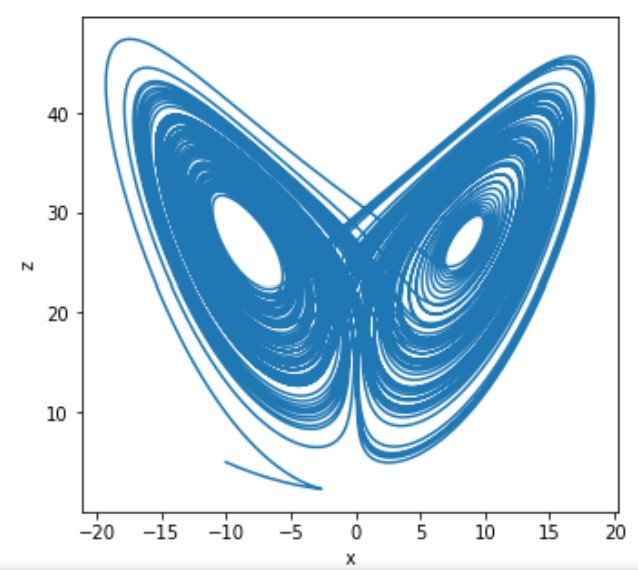
\includegraphics[width=0.5\textwidth]{"images/butterfly.jpg"}
	\end{center}
	\noindent Few remarks about the attractor:
	\begin{enumerate}[label=\textbullet]
		\item The trajectory seems to cross several times, but this is just an illusion of the projection of the three dimensional trajectory on a two dimensional plane. In 3D, there are no crossings.
		\item The number of circuits made on either side varies unpredictably from one cycle to the next. The sequence of the number of circuits in each lobe has many of the characteristics of a random sequence.
		\item When the trajectory is viewed in 3 dimensions, it appears to settle onto a thin set that looks like a pair of butterfly wings. We call this attractor a strange attractor and it can be shown schematically as :
		\begin{center}
			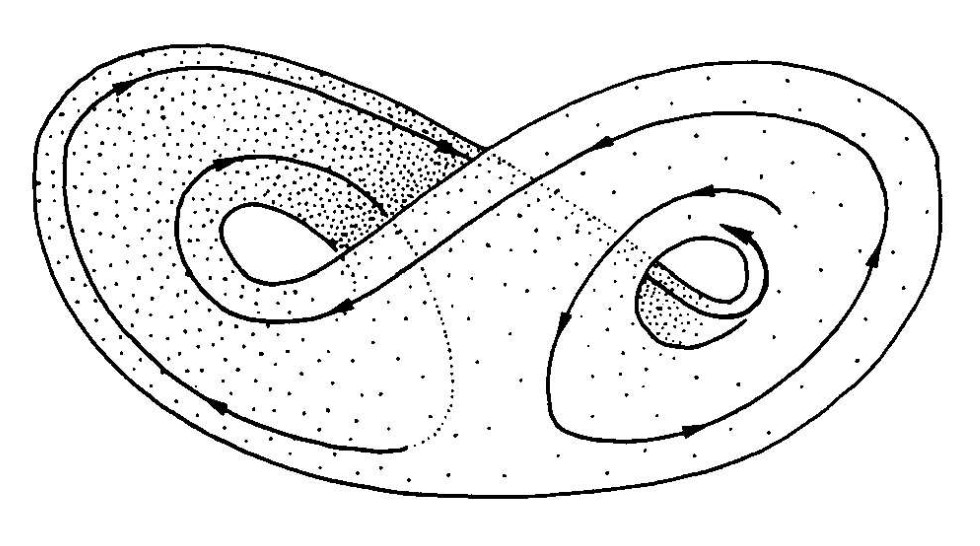
\includegraphics[width=0.5\textwidth]{"images/butterfly3D.jpg"}
		\end{center}
	\end{enumerate}
	
	\noindent The uniqueness theorem \cite{partie1_ref2} means that trajectories cannot cross or merge, hence the two surfaces of the strange attractor can only appear to merge. Lorenz concluded that “there is an infinite
	complex of surfaces” where they appear to merge. Today this “infinite complex of surfaces” would be called a fractal, which is a set of points with zero volume but infinite surface area.
	
	\noindent The term attractor is also difficult to define in a rigorous way. Loosely, an attractor is a set of points to which all neighbouring trajectories converge. Stable fixed points and
	stable limit cycles are examples. Nobody has yet proved that the Lorenz attractor is truly an attractor. Finally we define a strange attractor to be an attractor that exhibits sensitive dependence on initial conditions \cite{partie1_ref2}.
	
	\subsection{Chaos theory}
	
	In 1961, Lorenz was working with a simplified system that represented the atmosphere, with 12 variables. A computer was used to calculate the values for each instant by applying the equations to the values from the previous moment. In some cases, Lorenz’s team needed to re-start the simulation. Since the equations was the same, they expected to see the same results but sometimes they didn’t. At first, they thought that the problem was coming from the computer, but actually the error came from the fact that the computer was storing numbers with six decimal places but it was only printing the number with 3 decimal places, so the values that Lorenz put into the computer had tiny errors. So he discovered that in some systems, tiny changes in the initial conditions can lead to big changes in time.
	
	\noindent This effect was later named "butterfly effect". The "butterfly effect" refers to a system that is very sensitive to the initial condition, which is why these systems are very difficult to predict over time. This idea gave birth to the notion of a butterfly flapping its wings in a region of the world and causing a tornado.
	The Lorenz equations are a chaotic system, which means that this type of system is roughly defined by sensitivity to initial conditions: infinitesimal differences in initial conditions of the system result in large differences in behavior.
	
	\section{Numerical resolution of the Lorenz System with different methods}
	\label{sec4}
	
	We consider $f : [0; T] \times \mathbb{R}^n \rightarrow \mathbb{R}^n$ a continuous function. For $X_0\in \mathbb{R}^n$, the problem is to find  $X\in C^1([0,T],\mathbb{R}^n)$ a solution for the differential equation:
	
	$$\left\{\begin{aligned}
		X'&=f(t,X), \\
		X(0)&=X_0.
	\end{aligned}\right.$$
	
	\noindent To solve the Lorenz problem we will have:
	
	$$X'=\begin{pmatrix}
		x' \\
		y' \\
		z'
	\end{pmatrix}, \quad X=\begin{pmatrix}
		x \\
		y \\
		z
	\end{pmatrix} \quad \test{and} \quad f(t,X)=\begin{pmatrix}
		\sigma(y-x) \\
		x(r-z)-y \\
		xy-bz
	\end{pmatrix}$$.
	
	\noindent After discretizing the problem in time, we can implement different methods to solve the ODE. The methods are the following and will be described in more detail in the following parts: explicit Euler, implicit Euler and Runge Kutta (order 4). We will also use a scipy function and finally compare all our methods.
	
	\subsection{Discretization}
	
	To solve the problem, we will use the finite difference method. We will start by slicing the interval $[0,T]$ in $N+1$ discretization points (so $N$ intervals). Let $t_n=n\Delta t$ the discretization timed with $\Delta t=T/N$ the times step. Then, we denote by $X_n=X(t_n)$ the discretization points. So for $n=\{0,\dots,N\}$, we will have:
	
	$$\left\{\begin{aligned} 
		x_n&=x(t_n)=x(n\Delta t), \\
		y_n&=y(t_n)=y(n\Delta t), \\
		z_n&=z(t_n)=z(n\Delta t).
	\end{aligned}\right.$$
	
	\noindent By Taylor's theorem, we get :
	
	$$\begin{aligned}
		&&X(t+\Delta t)&=X(t)+\Delta t X'(t) + O(\Delta t^2) \\
		\Rightarrow&& \quad X'(t)&=\frac{X(t+\Delta t)-X(t)}{\Delta t} + O(\Delta t) \\
		\Rightarrow&& \quad \partial_t X_n&\approx\frac{X_{n+1}-X_n}{\Delta t} \\
	\end{aligned}
	$$	
	
	\subsection{Explicit Euler}
	
	The explicit Euler method is written :
	
	$$X_{n+1}=X_n+\Delta t f(t_n,X_n)$$,
	
	\noindent which will give us:
	
	$$\left\{\begin{aligned} 
		x_{n+1}&=\sigma\Delta t y_n+(1-\sigma\Delta t) x_n ,\\
		y_{n+1}&=\Delta t x_n(r-z_n)(1-\Delta t)y_n ,\\
		z_{n+1}&=\Delta t x_ny_n+(1-b\Delta t)z_n.
	\end{aligned}\right.$$
	
	\subsection{Implicit Euler}
	
	The implicit Euler method is written :
	
	$$X_{n+1}=X_n+\Delta t f(t_{n+1},X_{n+1}),$$
	
	\noindent which will give us:
	
	$$\left\{\begin{aligned} 
		x_{n+1}&=x_n+\Delta t\sigma(y_{n+1}-x_{n+1}), \\
		y_{n+1}&=y_n+\Delta t x_{n+1}(r-z_{n+1})-y_{n+1}, \\
		z_{n+1}&=z_n+\Delta tx_{n+1}y_{n+1}-\Delta tbz_{n+1}.
	\end{aligned}\right.$$
	
	\begin{enumerate}[label=\textbullet]
		\item First, we isolate the $n+1$ terms on the left and the $n$ terms on the right:
		
		$$\left\{\begin{aligned} 
			(1+\Delta t\sigma)x_{n+1}-\Delta t\sigma y_{n+1}&=x_n, \\
			-\Delta t(r-z_{n+1})x_{n+1}+(1+\Delta t)y_{n+1}&=y_n, \\
			-\Delta ty_{n+1}x_{n+1}+(1+\Delta tb)z_{n+1}&=z_n,
		\end{aligned}\right.$$
		
		\item We can then linearize the terms 
		
		$$\begin{aligned}
			x_{n+1}y_{n+1}&\approx x_{n+1,k+1}y_{n+1,k}, \\
			x_{n+1}z_{n+1}&\approx x_{n+1,k+1}z_{n+1,k}.
		\end{aligned}$$ 		
		\noindent Then, we get :
		
		$$\left\{\begin{aligned} 
			(1+\Delta t\sigma)x_{n+1,k+1}-\Delta t\sigma y_{n+1,k+1}&=x_n ,\\
			-\Delta t(r-z_{n+1,k})x_{n+1,k+1}+(1+\Delta t)y_{n+1,k+1}&=y_n , \\
			-\Delta ty_{n+1,k}x_{n+1,k+1}+(1+\Delta tb)z_{n+1,k+1}&=z_n ,
		\end{aligned}\right.$$
		
		\item We can then put in matrix form  $M(X_{n+1,k})X_{n+1,k+1}=X_n$ with :
		
		$$M(X_{n+1,k})=\begin{pmatrix}
			1+\Delta t\sigma & -\Delta t\sigma & 0 \\
			-\Delta t(r-z_{n+1,k}) & 1+\Delta t & 0 \\
			-\Delta ty_{n+1,k} & 0 & 1+\Delta tb
		\end{pmatrix},$$
		$$X_{n+1,k+1}=\begin{pmatrix}
			x_{n+1,k+1} \\
			y_{n+1,k+1} \\
			z_{n+1,k+1}
		\end{pmatrix} \quad \text{and} \quad X_n=\begin{pmatrix}
			x_n \\
			y_n \\
			z_n
		\end{pmatrix} $$
	\end{enumerate}

	\noindent We make a loop on the $k$ iterator until we have, for $\epsilon>0$ chosen in advance:
	
	$$\frac{||x_{n+1}^{k+1}-x_{n+1}^k||}{||x_{n+1}^k||}<\epsilon$$
	
	\subsection{Runge Kutta}
	\label{sec4.4}
	
	\begin{enumerate}[label=\textbullet]
		\item \textbf{Runge Kutta (order 4) :} \\
		The Runge Kutta method of order 4 is written :
		
		$$X_{n+1}=X_n+\frac{\Delta t}{6}\left(K_1+2K_2+2K_3+K_4\right) ,$$
		
		\noindent where 
		
		$$\left\{\begin{aligned}
			K_1&=f(t_n,X_n) , \\
			K_2&=f\left(t_n+\frac{\Delta t}{2},X_n+\frac{1}{2} K_1\Delta t\right) , \\
			K_3&=f\left(t_n+\frac{\Delta t}{2},X_n+\frac{1}{2} K_2\Delta t\right) , \\
			K_4&=f\left(t_n+\Delta t,X_n+K_3\Delta t\right) .
		\end{aligned}\right.$$
		\item \textbf{Scipy function :} \href{https://docs.scipy.org/doc/scipy/reference/generated/scipy.integrate.solve_ivp.html#scipy.integrate.solve_ivp}{scipy.integrate.solve\_ivp} \\
		This function solve an initial value problem for a system of ODEs. We can chose the numerical method to be used ie the argument "method" which is by default RK45. 
	\end{enumerate}
	
	\subsection{Comparing methods}
	
	\begin{enumerate}[label=\textbullet]
		\item First, we had to implement a function allowing to plot a 2D graph representing $x$ versus $y$, then a 2D graph representing $x$ versus $z$ and finally a 3D graph of the solution. Then, we implemented the different methods described above and we checked visually that they worked correctly. Here are the graphs obtained with the following parameters :
		\begin{center}
			$\sigma=10,\quad \beta=8/3 \quad r=9/10$ ,\\
			$X_0=(-10,10,5)$ ,\\
			$N=5000, \quad T=100 .$
		\end{center}
		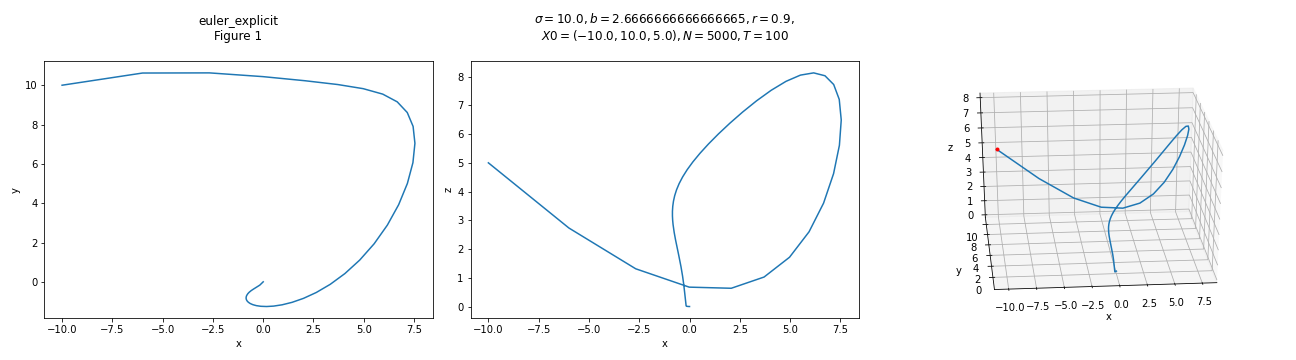
\includegraphics[width=\textwidth]{"images/euler_explicit.png"}
		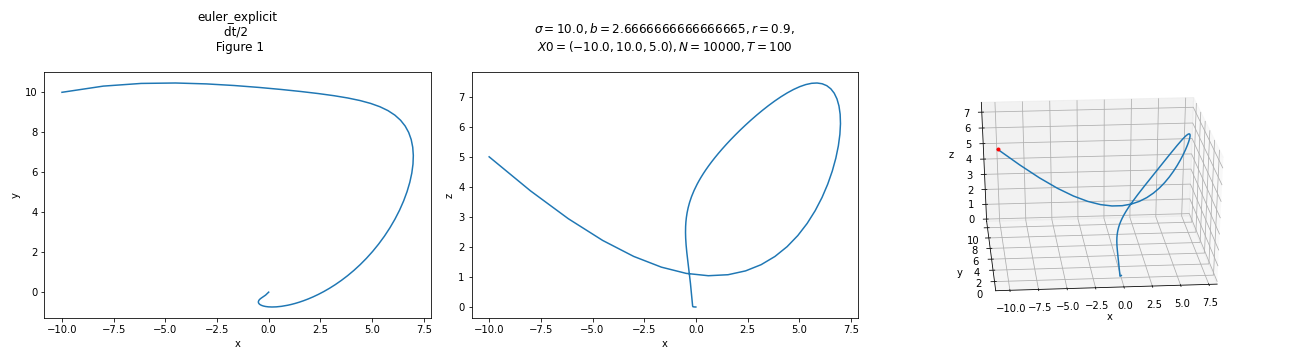
\includegraphics[width=\textwidth]{"images/euler_explicit_dt2.png"}
		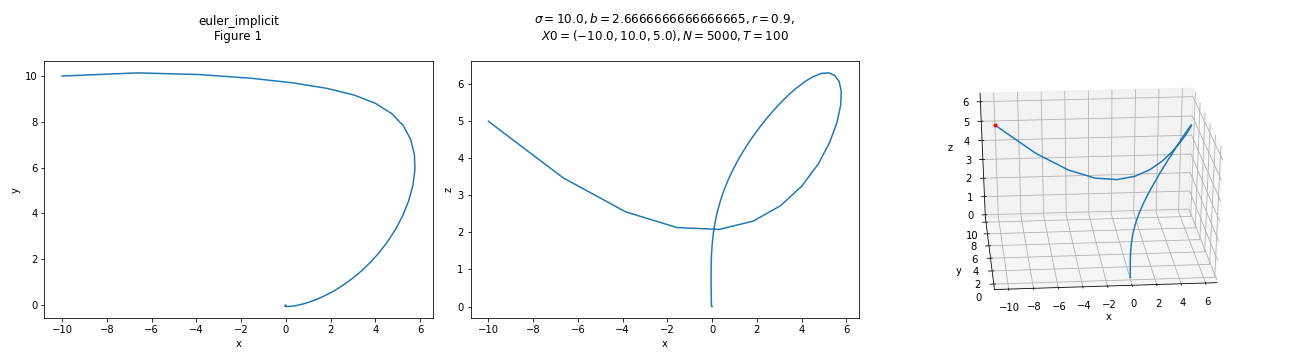
\includegraphics[width=\textwidth]{"images/euler_implicit.png"}
		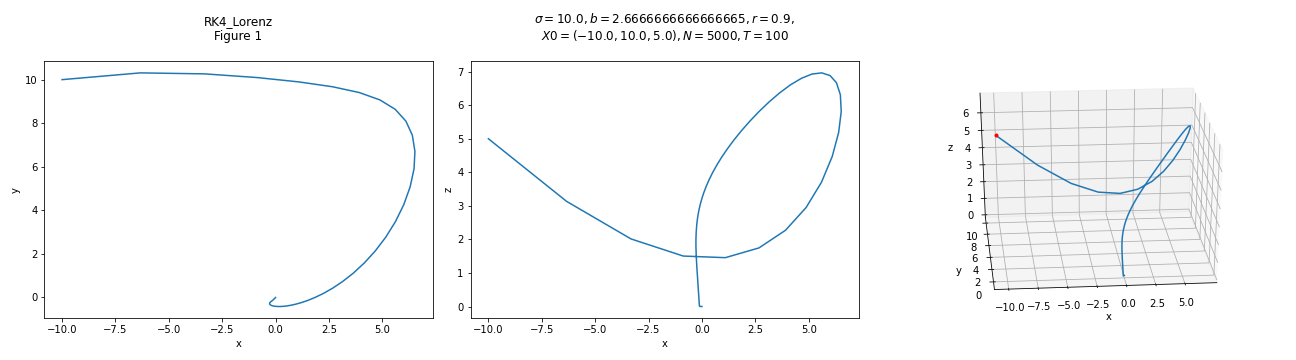
\includegraphics[width=\textwidth]{"images/RK4_Lorenz.png"}
		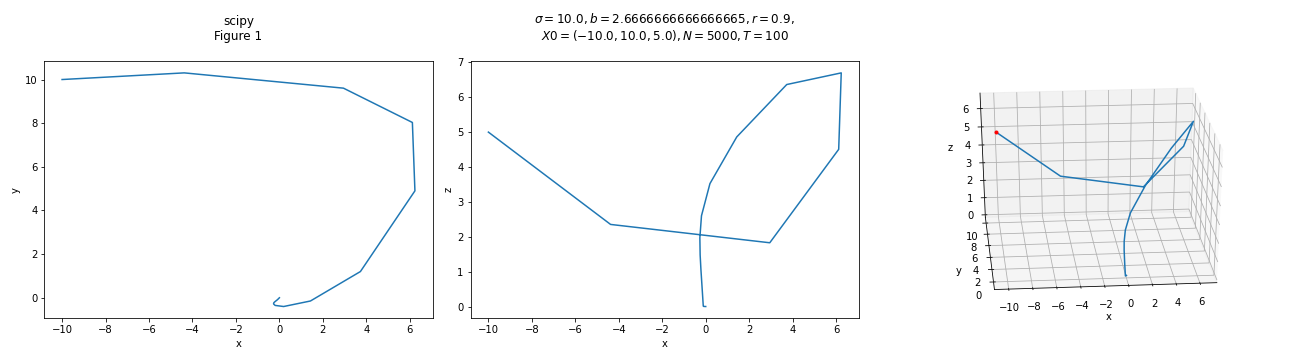
\includegraphics[width=\textwidth]{"images/scipy.png"}
		\item Then, we compared the execution times of these different methods (until $T=100$). Here is what we get with the same parameters : \\
		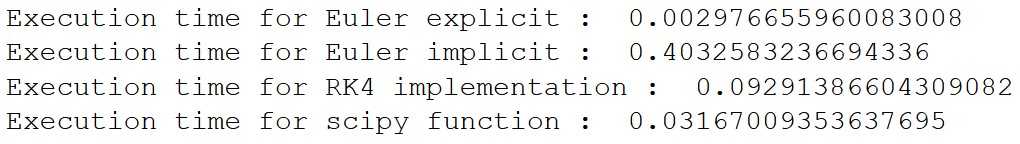
\includegraphics[width=0.7\textwidth]{"images/execution_times.jpg"} \\
		It seems that the explicit Euler method is the fastest, followed by the scipy function. \\
		We can see that implicit Euler is takes more times than the others. This is probably due to the loop on $k$ for each $n$. \\
	\end{enumerate}

	%\noindent For the next part of the project, we choose to work with the Runge kutta method.
	
	\newpage
	
	\begin{frame}{What is the parareal method ?}
	
	\begin{enumerate}[\textbullet]
		\item parallel-in-time integration method, introduced in 2001 by Lions, Maday and Turinici
		\item computes the numerical solution for multiple time steps in parallel
		\item categorized as a parallel-across-the-steps method 
	\end{enumerate}

\end{frame}

\begin{frame}{Objectives for parareal method}
	
	\begin{enumerate}[\textbullet]
		\item Implement the parareal method in C++ and :
		\begin{itemize}
			\item Test the method (with oscillator)
			\item Check convergence and stability results
			\item Check speed-up and efficiency 
		\end{itemize}
		\item Implement the resolution of the heat equation in C++ with Feel++ \\
		$\Rightarrow \quad $ Implement the resolution of the Laplace equation in C++ with Feel++ \\
		\item Use the previous implementation of the heat equation with the parareal method
		\item Check the convergences/accuracies of the method
	\end{enumerate}
	
\end{frame}


\subsection{Theory}

\begin{frame}{Generalities of the parareal method}
	Time decomposition :
	\begin{enumerate}[\textbullet]
		\item $[t_0,T]=[t_0,t_1]\cup\dots\cup[t_{P-1},t_P]$ with $t_P=T$ and $P=$ number of processes
	\end{enumerate}

	\; \\

	\begin{minipage}{\linewidth}
		Notations :
		\begin{enumerate}[\textbullet]
			\item $F$ : high accuracy integrator, \quad $\Delta t_F$ : time step \\
			$G$ : low accuracy integrator, \quad $\Delta t_G$ : coarse time step
			\item $U_j^k, j\in\{0,\dots,P\}$ : initial point at time $t_j$ and at iteration $k$.
		\end{enumerate}
	\end{minipage} \\
	\begin{enumerate}[\textbullet]
		\item $F(U_{j-1}^k), j\in\{1,\dots,P\}$ : value of the fine integrator at $t_j$ starting by $U_{j-1}^k$ (resp. $G(U_{j-1}^k)$)
	\end{enumerate}
	\begin{minipage}{\linewidth}
		\centering
		\qquad \qquad \qquad \qquad \qquad \qquad \qquad 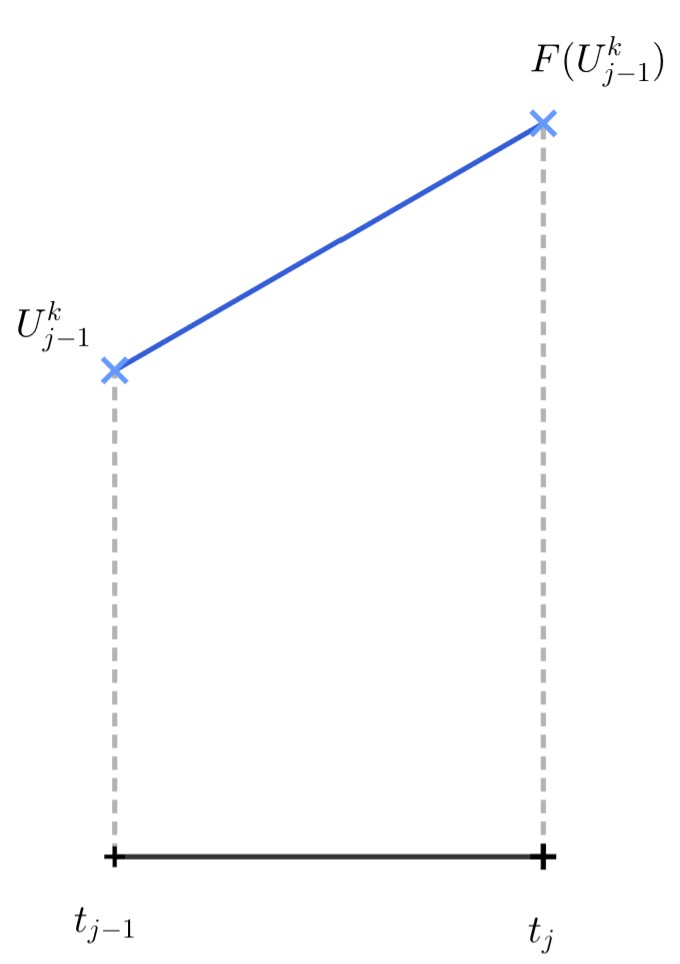
\includegraphics[width=0.35\linewidth]{images/parareal/explane_F.jpg}
	\end{minipage}
	
\end{frame}

\begin{frame}[allowframebreaks]{Explanation of the parareal method}
	\begin{figure}
		\centering
		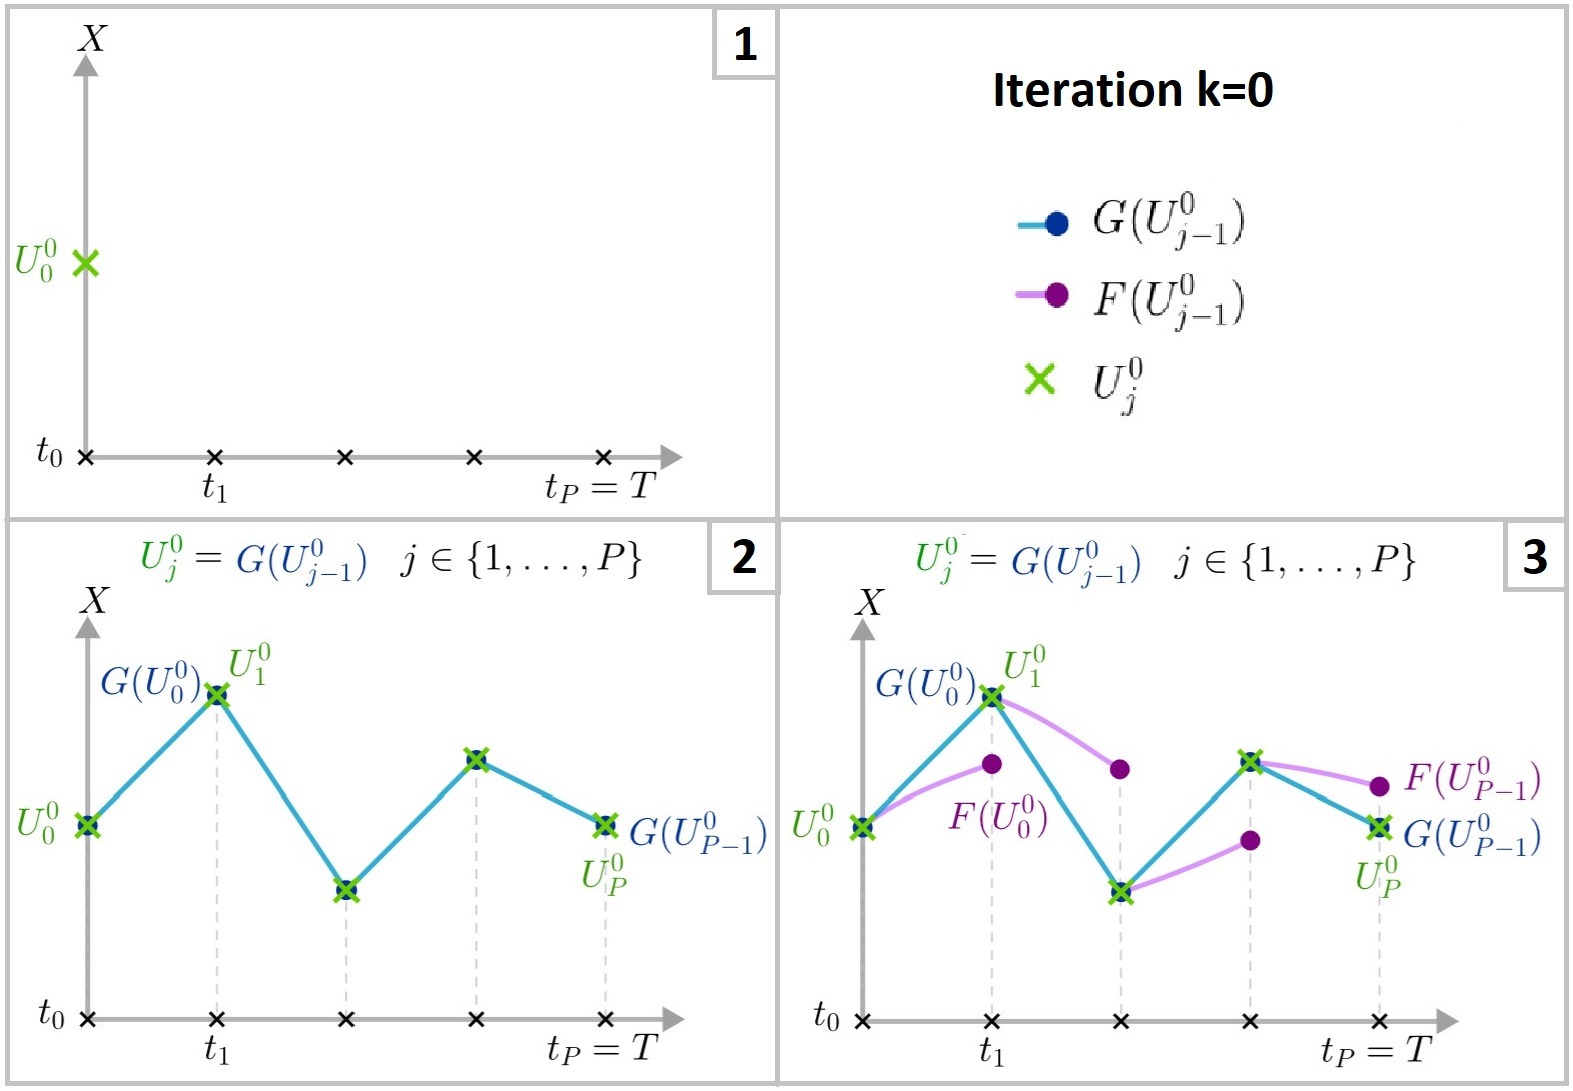
\includegraphics[width=0.6\linewidth]{images/parareal/parareal_k0.jpg}
		\caption{Explanation of the parareal method at iteration $k=0$ (step 1 to 3)}
	\end{figure}
	\begin{figure}
		\centering
		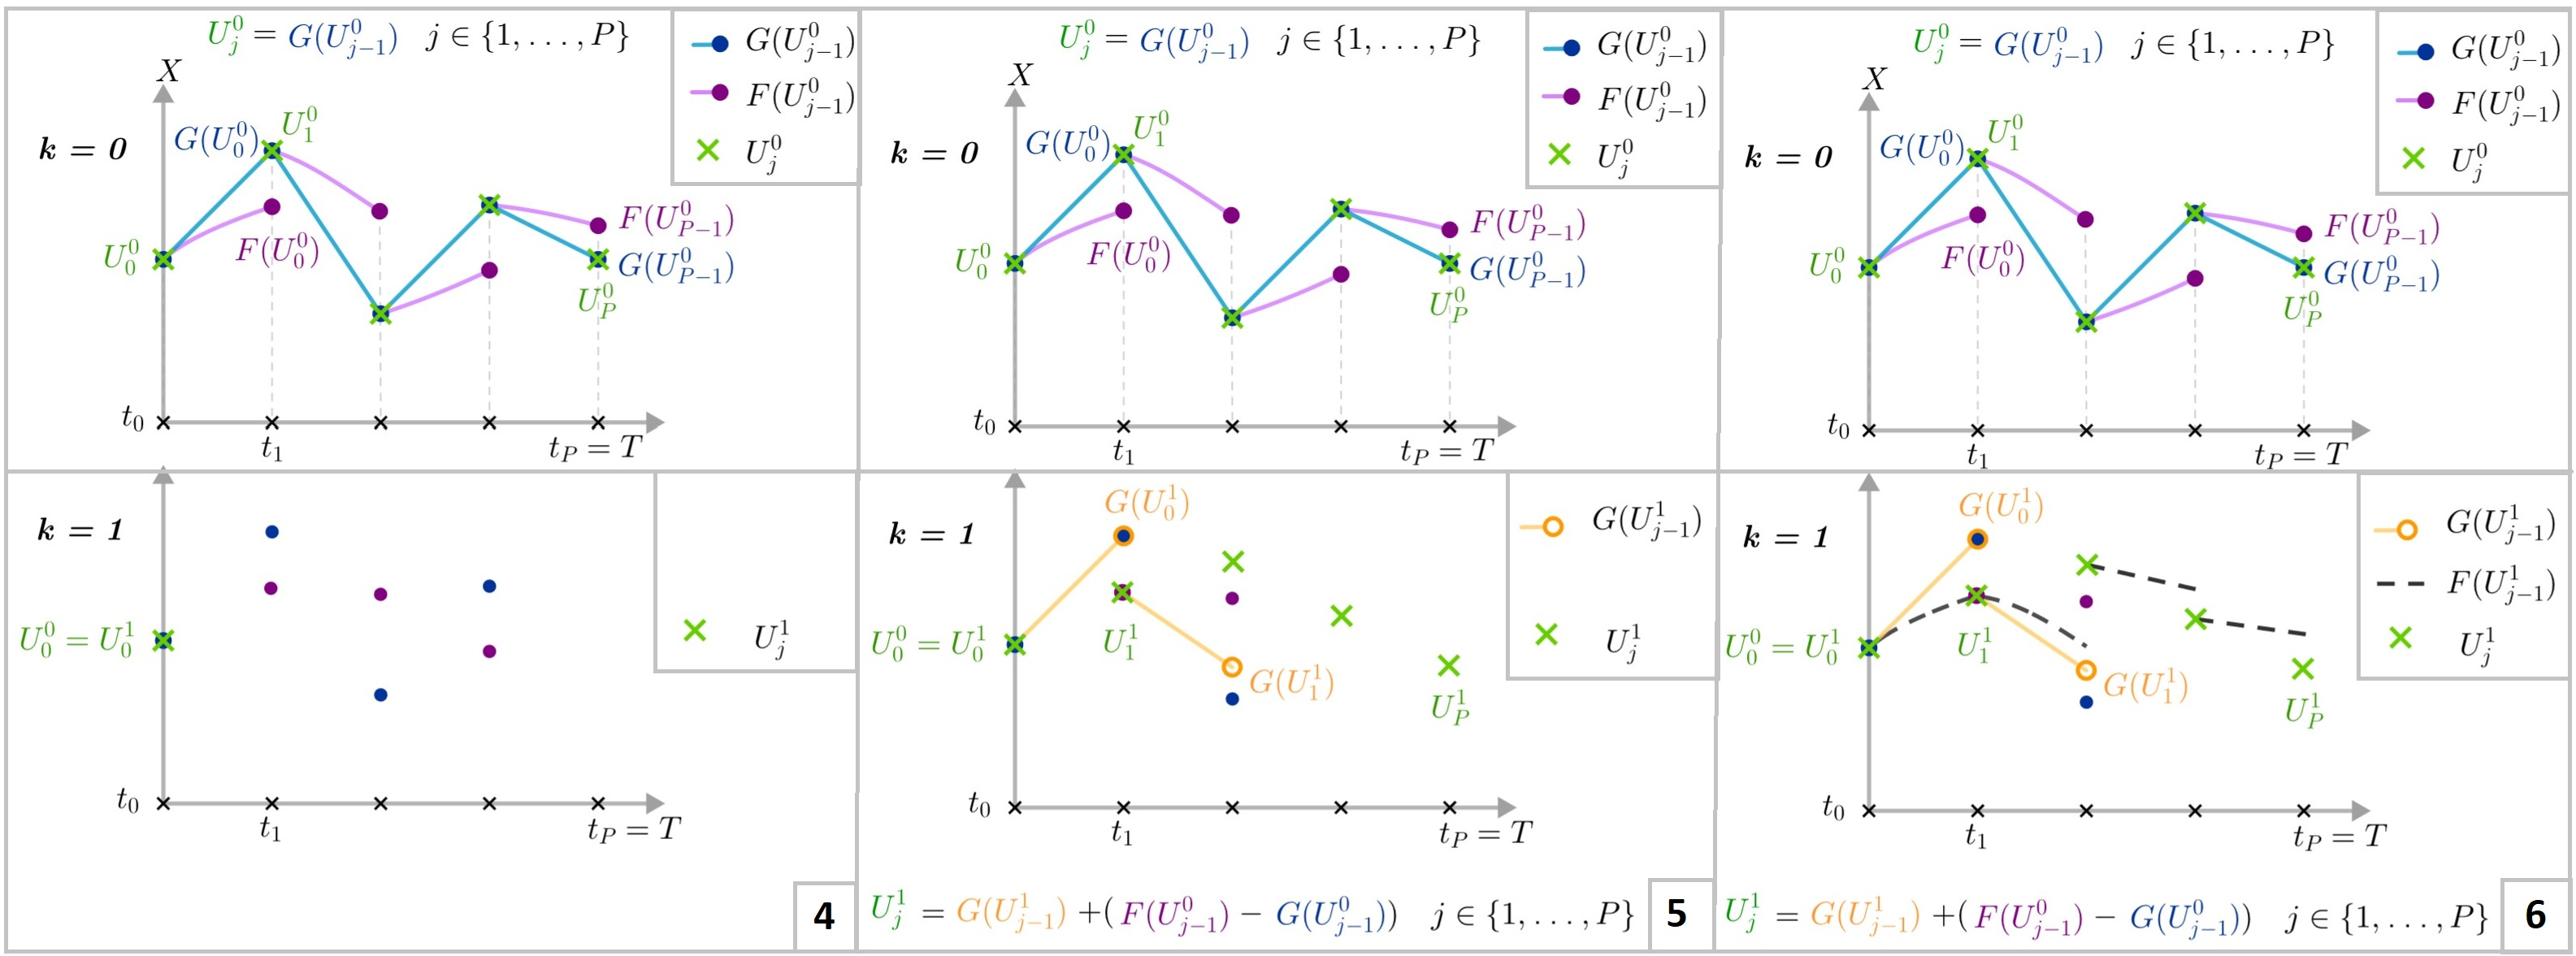
\includegraphics[width=0.9\linewidth]{images/parareal/parareal_k1.jpg}
		\caption{Explanation of the parareal method at iteration $k=1$ (step 4 to 6)}
	\end{figure}
	\small
	We have at iteration $k$ : \qquad	$U_j^k=G(U_{j-1}^k)+(F(U_{j-1}^{k-1})-G(U_{j-1}^{k-1}))$
\end{frame}

\begin{frame}{Example with the Lorenz system}
	\centering
	$\sigma=10, \quad b=\frac{8}{3}, \quad r=28, \quad X_0=(5,5,5), \quad t_0=0, \quad T=20$
	$P=4,\quad \Delta t_G=0.1, \quad \Delta t_F=0.01$
	\begin{figure}
		\centering
		\begin{minipage}{0.48\linewidth}
			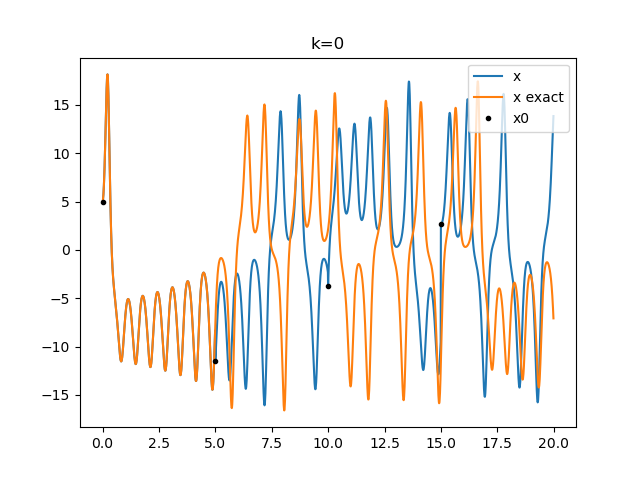
\includegraphics[width=\linewidth]{"images/parareal/lorenz_sol_0.png"}
		\end{minipage}
		\begin{minipage}{0.48\linewidth}
			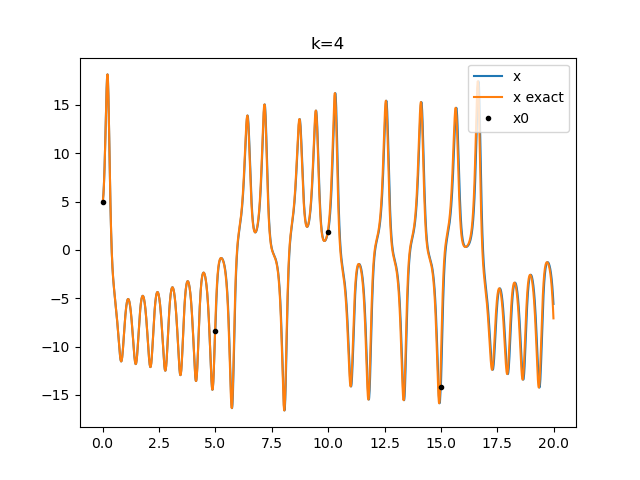
\includegraphics[width=\linewidth]{"images/parareal/lorenz_sol_4.png"}
		\end{minipage}
		\caption{Solution of the Lorenz system at the first and the last iteration (with C++)}
	\end{figure}
\end{frame}

\begin{frame}{Order of the parareal method}
	The parareal method is of order k if there is a constant $c_k$ such that :
	\begin{equation*}
		\forall j\in\{0,\dots,P-1\} \qquad \mathcal{E}(j,k)\le c_k(\Delta t_G)^k
	\end{equation*}
	with
	$$\mathcal{E}(j,k)=|U_j^k-U_{ex}(t_j)|+\max_{t\in[t_j,t_{j+1}]}|U_k(t)-U_{ex}(t)|$$
	\begin{figure}
		\centering
		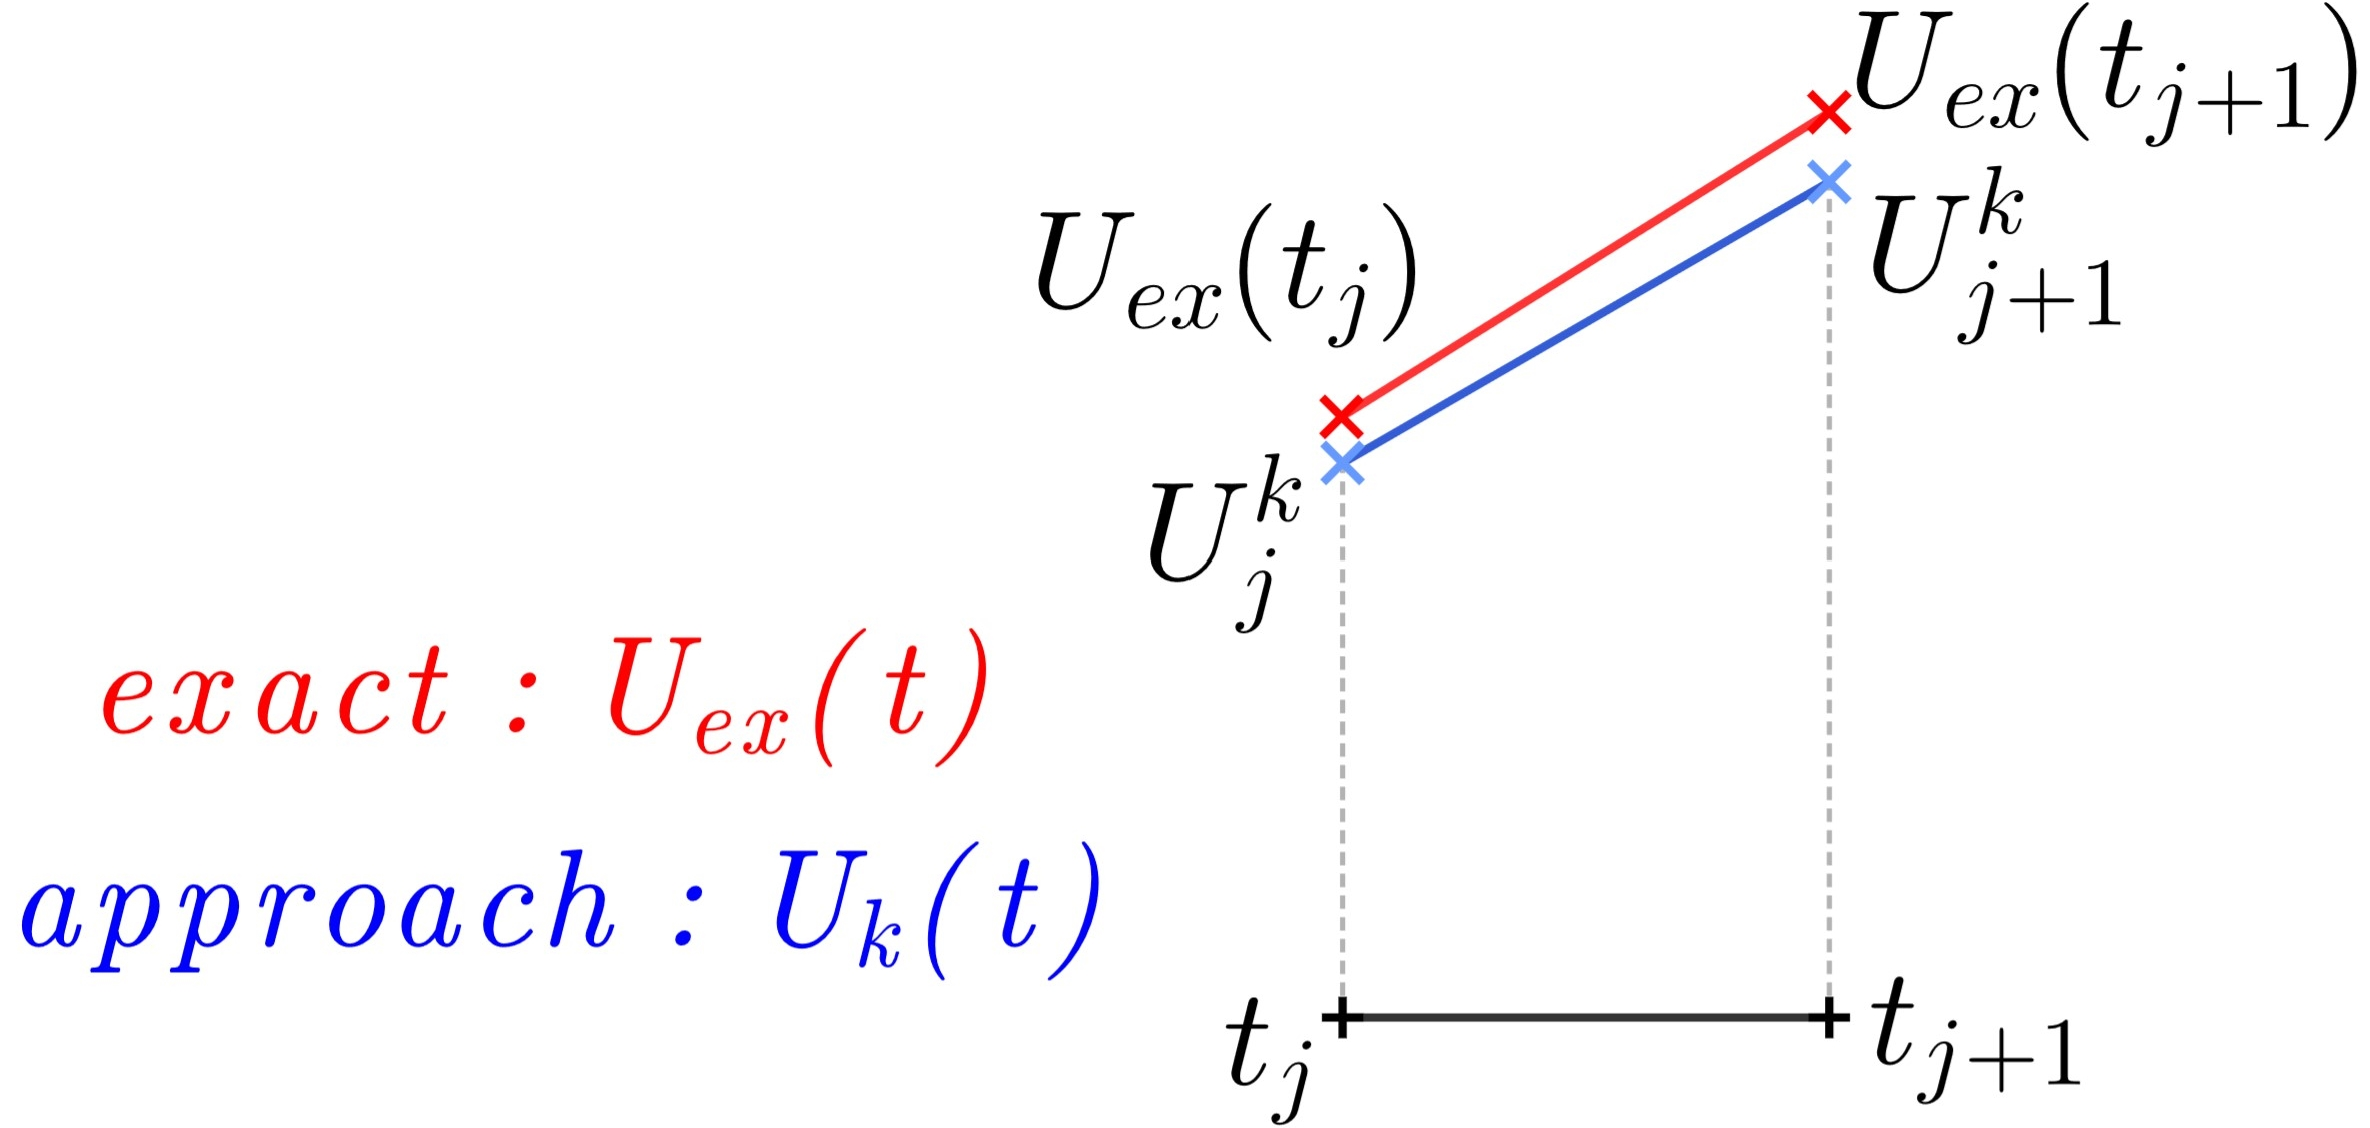
\includegraphics[width=0.62\linewidth]{images/parareal/explane_order.jpg}
		\caption{Explanation of the order property}
	\end{figure}
\end{frame}


\begin{frame}{Harmonic oscillator}
	
	$$P=3, \quad x(0)=0,\quad v(0)=1, \quad\omega_0=5, \quad x_0=\frac{-1}{5}, \quad \phi_0=\frac{\pi}{2}$$
	
	\begin{minipage}{0.45\linewidth}
		\begin{figure}
			\centering
			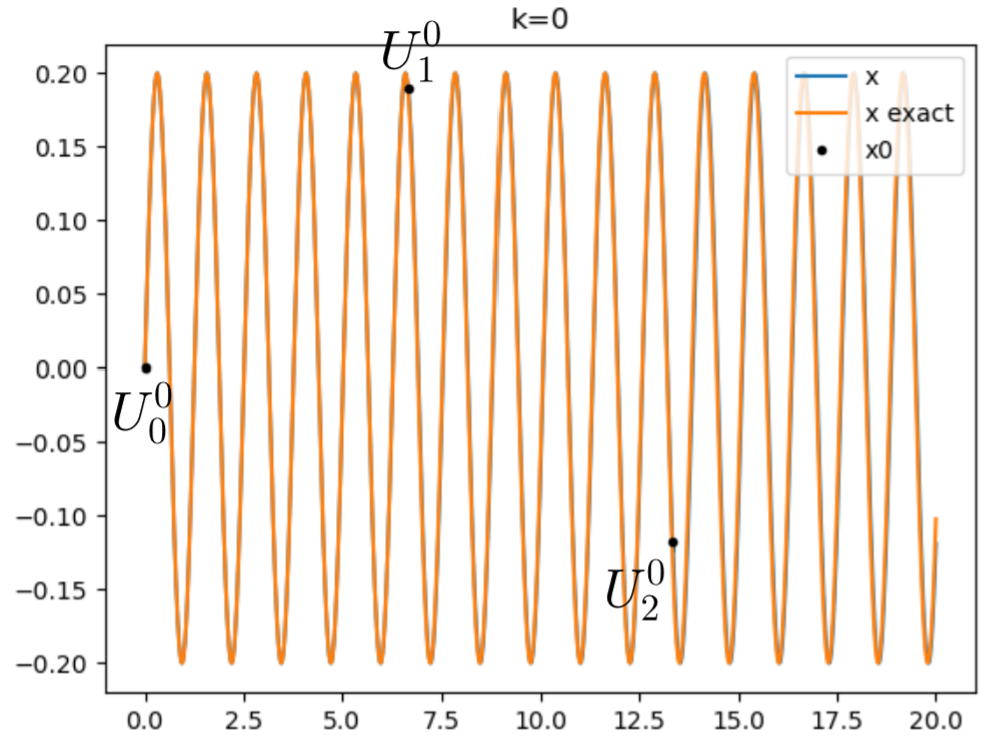
\includegraphics[width=\linewidth]{"images/parareal/osci_sol.png"}
			\caption{Parareal method applied to the harmonic oscillator (with C++)}
		\end{figure}
	\end{minipage} \; \qquad
	\begin{minipage}{0.45\linewidth}
		\begin{figure}
			\centering
			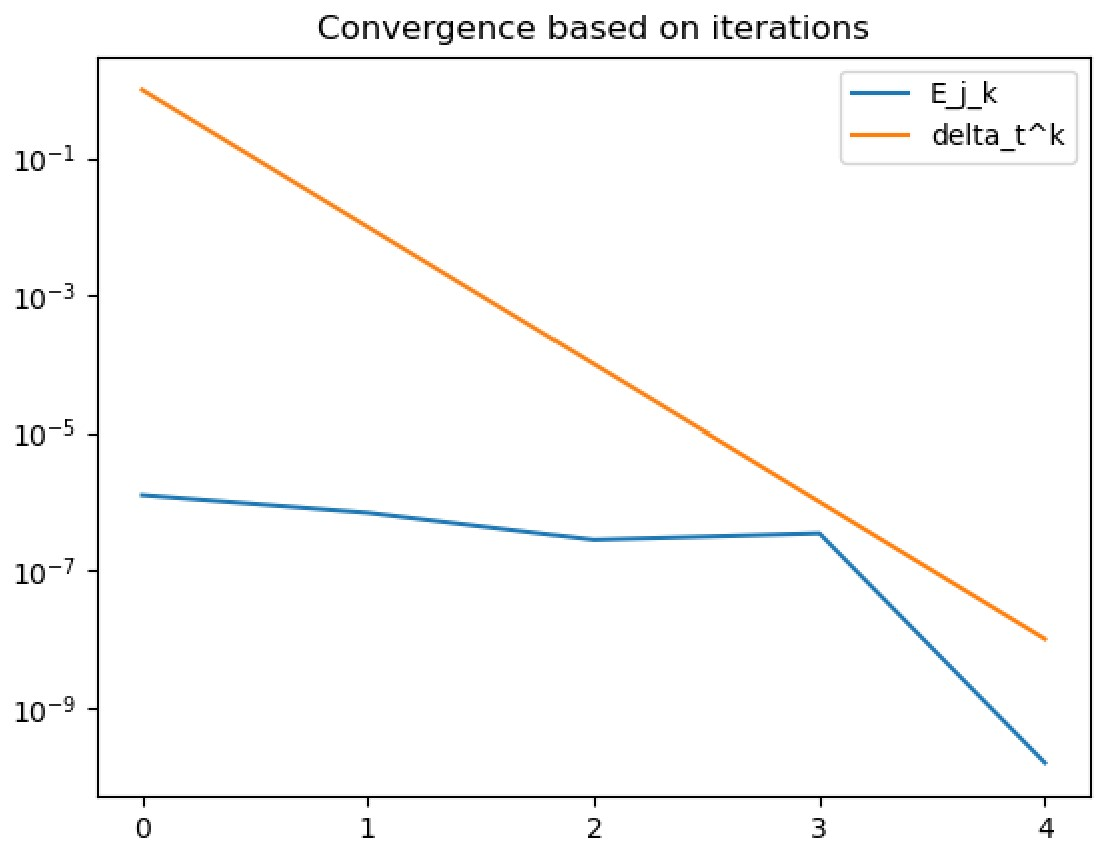
\includegraphics[width=\linewidth]{"images/parareal/osci_cvg_1.jpg"}
			\caption{Convergence property of parareal method with the harmonic oscillator (with Python)}
		\end{figure}
	\end{minipage}
	
\end{frame}

\begin{frame}{Speed-up ?}
	\begin{enumerate}[\textbullet]
		\item Why use this method ? \\
		Useful if the number of iteration is lower than $P$. \\
		
		\item We can see that the implementation of the method in C++ is considerably faster than in Python. \\
		
		\item Speed-up when we increase the number of processes $P$ ? \\
		With Python :
		\begin{table}[H]
			\centering
			\begin{tabular}{| c || c | c | c | c | c |}
				\hline
				\multirow{2}{1.5 cm}{$\Delta t$} & \multirow{2}{1.5 cm}{Seq (RK4)} & \multirow{2}{1.5 cm}{1 proc} & \multirow{2}{1.5 cm}{2 proc} & \multirow{2}{1.5 cm}{3 proc} &\multirow{2}{1.5 cm}{4 proc} \\
				& & & & & \\
				\hline 
				F : 0.00125 & \multirow{2}{1.5 cm}{1m19} & \multirow{2}{1.5 cm}{1m42} & \multirow{2}{1.5 cm}{39s} & \multirow{2}{1.5 cm}{32s} & \multirow{2}{1.5 cm}{29s} \\
				G : 0.0125 & & & & & \\	 
				\hline
			\end{tabular}
			\caption{Execution time for the Lorenz system with Python ($T=200$).}
			\label{time}
		\end{table}
	\end{enumerate}
\end{frame}






\subsection{Solving PDEs with Feel++}

\begin{frame}{Heat equation}
	
	\textbf{The problem :}
	$$\left\{\begin{aligned}
		\frac{\partial u}{\partial t}-\Delta u &= f \quad&&(t_0,T)\times\Omega \\
		u&=0 \quad&&(t_0,T)\times\partial\Omega\\
		u&=u_0 \quad &&\{0\}\times\Omega
	\end{aligned}\right.$$

	It describes the time evolution of the temperature $u$ of a medium contained in $\Omega$ under an external heat source $f$; $u_0$ is the initial temperature.
	
\end{frame}

\begin{frame}{Laplacian equation}
	
	\textbf{The problem :}
	$$\left\{\begin{aligned}
		-\Delta u &= f \quad&&\Omega \\
		u&=g \quad&&\Gamma_D \\
		\frac{\partial u}{\partial n} &=h \quad &&\Gamma_N \\
		\frac{\partial u}{\partial n}+u &=l \quad &&\Gamma_R \\
	\end{aligned}\right.$$
	
	\textbf{Weak formulation :} \\
	Find $\; u:\Omega \mapsto \mathbb{R} \;$ such that $\; u\in H_0^1(\Omega) \;$ and
	$$\int_\Omega \nabla u \cdot \nabla v + \int_{\Gamma_R}uv = \int_\Omega fv + \int_{\Gamma_N}hv+\int_{\Gamma_R}lv \quad \forall v\in H_0^1(\Omega)$$
	
\end{frame}

\begin{frame}[allowframebreaks]{Example with Laplacian}
	$$\left\{\begin{aligned}
		-\Delta u &= f \quad&&\Omega \\
		u&=g \quad&&\Gamma_D \\
	\end{aligned}\right. \quad \text{with} \quad
	u_{exact}=g=x^2+y^2, \quad f=-\Delta u_{exact}=-4$$
	\begin{minipage}{0.31\linewidth}
		\begin{figure}
			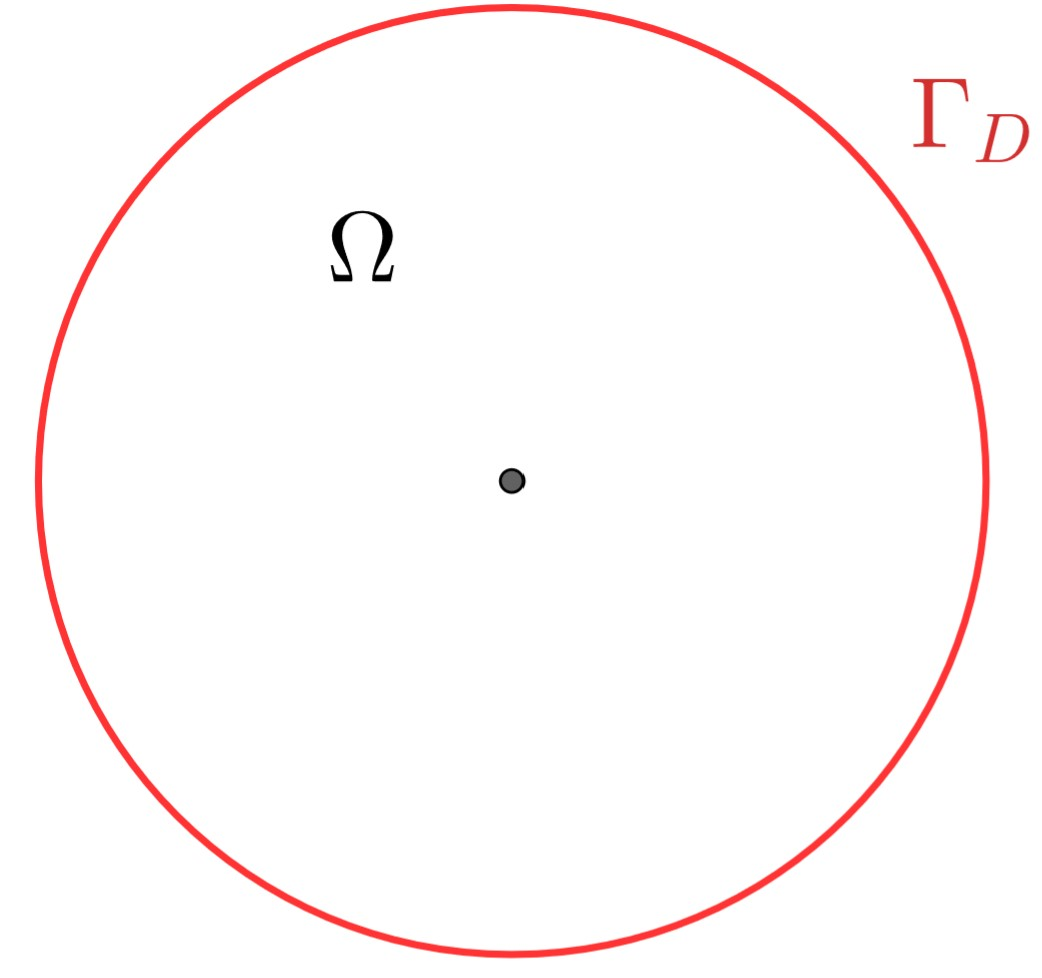
\includegraphics[width=\linewidth]{"images/parareal/circle.jpg"}
			\caption{Geometry considered}
		\end{figure}
	\end{minipage} \quad
	\begin{minipage}{0.31\linewidth}
		\begin{figure}
			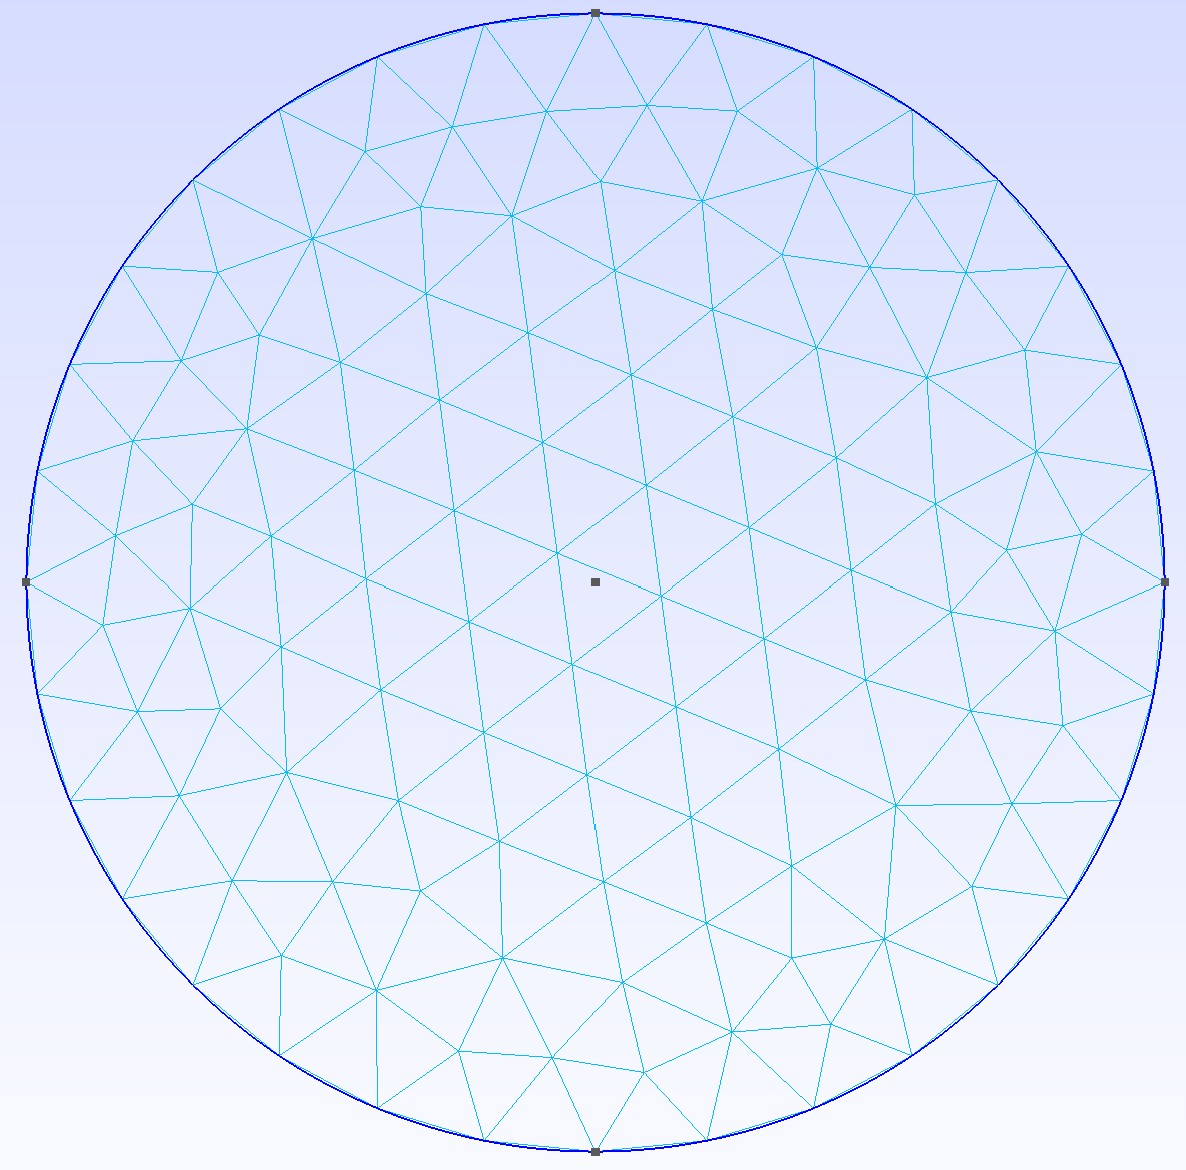
\includegraphics[width=\linewidth]{"images/parareal/circle_mesh.jpg"}
			\caption{Mesh of the geometry (with Dirichlet Boundary condition)}
		\end{figure}
	\end{minipage} \quad
	\begin{minipage}{0.31\linewidth}
		\begin{figure}
			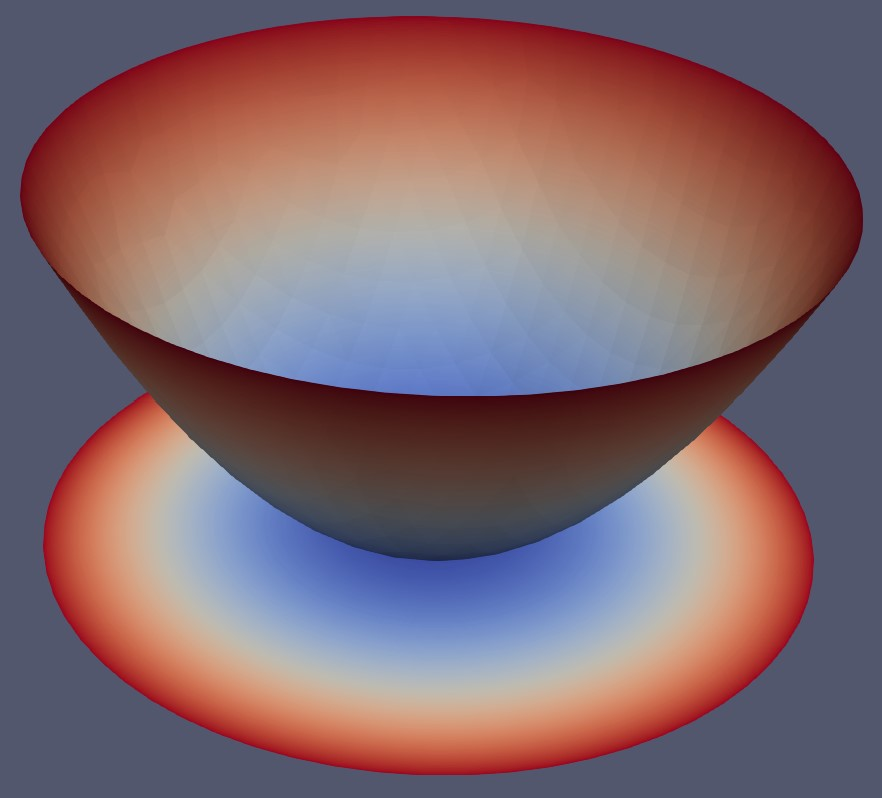
\includegraphics[width=\linewidth]{"images/parareal/circle_result.jpg"}
			\caption{Result (with Paraview)}
		\end{figure}	
	\end{minipage}

	\newpage
	\centering
	$||u-u_h||_{L^2}\sim h^2 \qquad \qquad ||u-u_h||_{H^1}\sim h^1 $
	\begin{figure}
		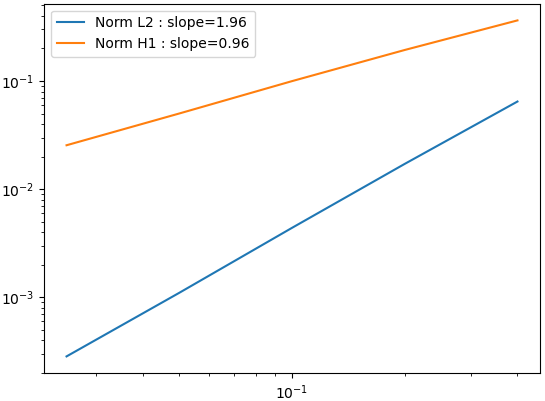
\includegraphics[width=0.52\linewidth]{"images/parareal/cvg_laplacian.png"}
		\caption{Convergence order for the Laplacian problem.}
	\end{figure}
\end{frame}

\begin{frame}{Back to the heat equation}
	\textbf{Weak formulation :} \\
	Find $\; u:(t_0,T)\times\Omega \mapsto \mathbb{R} \;$ such that $\; u(t,\cdot)\in H_0^1(\Omega) \;$ and
	$$\int_\Omega \frac{\partial u}{\partial t}(t,x)v(x)dx+\int_\Omega \nabla u(t,x)\cdot\nabla v(x)dx = \int_\Omega f(t,x)v(x)dx \quad \forall v\in H_0^1(\Omega)$$
	for almost every $t\in(0,T)$. \\
	
	
\end{frame}

\begin{frame}{Back to the heat equation}
	\textbf{Weak formulation :} \\
	Find $\; u:(t_0,T)\times\Omega \mapsto \mathbb{R} \;$ such that $\; u(t,\cdot)\in H_0^1(\Omega) \;$ and
	$$\boxed{\int_\Omega \frac{\partial u}{\partial t}(t,x)v(x)dx}+\int_\Omega \nabla u(t,x)\cdot\nabla v(x)dx = \int_\Omega f(t,x)v(x)dx \quad \forall v\in H_0^1(\Omega)$$
	for almost every $t\in(0,T)$. \\ \; \\
	
	need to manage the temporal discretizations \\
	$\Rightarrow$ use of the Feel++ bdf (Backward differencing formula) class :
	
	$$\int_\Omega \frac{\partial u}{\partial t}(t,x)v(x)dx \simeq \int_\Omega \frac{u^{n+1}(x)-u^n(x)}{\Delta t}v(x)dx$$
	
	(Backward Euler scheme)
\end{frame}

\begin{frame}{Parareal method with the Heat equation}
	\textbf{Goal :} To have a function that solves the heat equation between $t_i$ and $t_j$ with an initial condition (by using the previous resolution in C++ with Feel++) and apply the parareal method to it.
\end{frame}






	
	\newpage
	
	\section{Data assimilation}

\subsection{Intro}
\noindent Data assimilation is nowadays widely used to make predictions in complex systems, for example in weather forecasting or ocean prediction. Data assimilation is a method that combines observations with the output of a model to improve a prediction. 
The main idea is to combine information from our model and from observations, in order to have a more reliable analysis. Sometimes what you are trying to improve in your model may not be in the same space as what you observe this is something that you need to consider while doing your assimilation. It is also important to control our output, it is up to us to decide which input is responsible for the error in our output. This means that there will be uncertainties coming from the model or from the observations, these uncertainties coming from our input will also translate into uncertainties in our output.
At the end of this data assimilation we will have obtained an output which will be an estimate of the unknown quantity called the state variables.
The best estimate is searched for as a linear combination of the background estimate and the observations:

$$x^a=Lx^b+Ky^0$$


\noindent Data assimilation methods are often split into two families: variational methods and statistical methods.
The first method, called variational methods, consists in minimizing a cost function with the least squares approach. 
\subsection{statistical approach}
\subsubsection{Kalman filter}
The Kalman filter method consists in looking for $x^a$ an analysis, this analysis will be a linear combination of what we already know, our model and our observations.
To explain this method let's consider that we observe a single quantity, an estimation of a scalar quantity at a point in space.For example we are observing the temperature in the middle of the room, and the model also simulate the temperature in the middle of the room.  We will then have :
$$x^a=x^b+K(y-x^b)$$
with $x^a$ the analysis, $x^b$ the background or model, and $y$ the observation. 
We suppose that the true state $x^t$ exists so:
$$x^a-x^t+K(y-x^t-x^b+x^t)$$
let's define the errors:
$$\begin{aligned}
&\epsilon^a=x^a-x^t \\
&\epsilon^b=x^b-x^t \\
&\epsilon^y=y-x^t \\
\end{aligned}$$
So we will have:
$$\epsilon^a=\epsilon^b+K(\epsilon^y-\epsilon^b)$$
If we have many realisation of these error, then we will have:
$$<\epsilon^a>=<\epsilon^b>+K(<\epsilon^y>-<\epsilon^b>)$$
We want to have the analysis error variance as low as possible .So we want to minimize $<(\epsilon^a)^2>$ with respect to $K$ ,this will give us:
$$<(\epsilon^a)^2>=<(\epsilon^b)^2>+K^2<(\epsilon^y-\epsilon^b)^2>+2K<\epsilon^b(\epsilon^y-\epsilon^b)^2>$$
$$2k<(\epsilon^y)^2+(\epsilon^b)^2>-2<(\epsilon^b)^2>=0$$
\noindent We assume that the errors in the background and observation are uncorrelated.
$$K=\frac{<(\epsilon^b)^2>}{<(\epsilon^b)^2>+<(\epsilon^y)^2>} \Rightarrow K=\frac{(\sigma^b)^2}{(\sigma^b)^2+(\sigma^y)^2} $$
where $(\sigma^y)^2$ is the observation error variance and $(\sigma^b)^2$ is the background or model error variance.
\newline\noindent If we have $(\sigma^y)^2=0$, $K=1$ and $x^a=y$  this means that the observation are perfect.
\newline\noindent And if $(\sigma^b)^2=0$, $K=0$ and $x^a=x^b$ this is equivalent to ignoring the observations.
\vspace*{5mm}
\newline Now that we have explained the method for solving $x^a$ let's try to generalize our formula.

$$\left\{\begin{aligned}
		&x^a=(I-KH)x^b+Ky^0=x^b+K(y^0-H(x^b)) \\
        &K=BH^T(HBH^T+R)^{-1} \\
	\end{aligned}\right.$$
With $K$ the gain or weight matrix, $(y^0-H(x^b))$ the innovation and $H$ the linear model of the observations.
This formulation is called the Best Linear Unbiased Estimator(BLUE) or least squares analysis.
The principle of the Kalman filter is based on this formulation. Here is a small figure which illustrates the Kalman filter.
\vspace*{5mm}
\begin{center}
		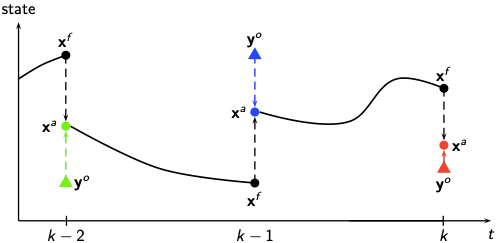
\includegraphics[width=0.8\textwidth]{"images/schema_kalman_filter.png"}
	\end{center}
The general idea consists in estimating the state at time $k$ from an estimate at time $k-1$ and measurements at time $k$.
We do the estimation in two steps:
\begin{enumerate}[label=\textbullet]
		\item Prediction of the state from the evolution model
		\item Correction of the prediction from the measurements
	\end{enumerate}

\subsubsection{Kalman filter algorithm}
For the notations we will use:

\noindent Vector:
 \begin{enumerate}[label=\textbullet]
		\item $k$ time index
		\item $x_{k}^{f}$ forecast state (background), forecast error covariance matrix $P_{k}^{f}$
		\item $x_{k}^{a}$ analyzed state (result of the assimilation process), analysis error covariance matrix $P_{k}^{a}$
	\end{enumerate}
\noindent Operators:
    \begin{enumerate}[label=\textbullet]
		\item model operator $x_{k+1}^{t} = M_{k,k+1}(x_{k}^{t})+ \eta
		_{k,k+1}$, model error $\eta
		_{k,k+1}$, covariance matrix $Q_k$
		\item observation operator $y_k^o = H_k (x^t ) + \epsilon_k^0$ , observation error $\epsilon^0$, covariance matrix $R_k$
	\end{enumerate}
\noindent The hypotheses necessary for the application of the Kalman filter are:
    \begin{enumerate}[label=\textbullet]
		\item Model and observations operators $M_{k,k+1}$ and $H_k$ are linear.
		\item Errors are unbiased, Gaussian, independent and white in time.
	\end{enumerate}
So finally we obtain the Kalman filter algorithm.
\begin{enumerate}[label=(\roman*)]
\item Initialization: $x_0^f$ and $P_0^f$ are given, equal to $x^b$ and $B$
\item BLUE:
$$\begin{aligned} &K_k=(H_kP_k^f)^T[H_k(H_kP_k^f)^T+R_k]^{-1} \\
&x_k^a=x_k^f+K_k(y_k^0-H_kx_k^f) \\
&P_k^a=(I-K_kH_k)P_k^f \\
\end{aligned}$$
\item Forecast step:
$$\begin{aligned} 
&x_{k+1}^f=M_{k,k+1}x_k^a \\
&P_{k+1}^f=M_{k,k+1}P_k^aM_{k,k+1}^T+Q_k\\
\end{aligned}$$
\end{enumerate}



\subsection{Variational approach}
\subsubsection{Minimizing a cost function}
\noindent In the previous part we have seen that there is a method called kalman filter which purpose is to make prediction with a model and observations, but there is also other method to make data assimilation like the variational assimilation, which solves the analysis problem through an optimisation (minimisation of a cost-function). This allows to solve the global problem in one go, and it is now widely used in the meteorological community. So variational data assimilation methods lead to the minimization of a cost function involving quadratic forms based on the both the background and observation covariance matrices. When the observation operator is linear the formulation of the cost function leads to the best the Best Linear Unbiased Estimation.An alternative way to define the analysis is to consider it as the maximum of the a posteriori p.d.f of the state given the observation and the background:
$$x^a=\arg\max_{x}p(x|y ~ and ~ x^b)$$
Using bayesian appreach $p(x|y)~\alpha~ p(y|x)p(x)$ we can simplify our probability by:
$$p(x|y ~ and ~ x^b)=\frac{p(y ~ and ~ x^b| x)p(x)}{p(y ~ and ~ x^b)}$$
We assume that observation and background errors are uncorrelated so we will have then:
$$(x|y ~ and ~ x^b)=p(y|x)p(x^b|x)$$
So we can define the cost function as:
$$J(x)=-log(p(y|x)p(x^b|x)+cst \\
=-log(p(y|x))-log(p(x^b|x))+cst$$
We can find the analysis by solving a minimization problem:
$$x^a=\arg\max_{x}J(x)$$
We assume that p.d.f are gaussien.
$$p(x^b|x)=(2\pi)^{-n/2}|B|^{-1/2}\exp({-\frac{1}{2}(x-x^b})^TB^{-1}(x-x^b))$$
$$p(y|x)=(2\pi)^{-m/2}|R|^{-1/2}\exp({-\frac{1}{2}(y-H(x)})^TR^{-1}(y-H(x)))$$
Which will lead us to:
$$J(x)=\frac{1}{2}(x^b-x)^TB^{-1}(x^b-x)+\frac{1}{2}(y-H(x))^TR^{-1}(y-H(x))$$
This is called the cost function of 3D-Var Approach.
\subsubsection{Generalisation of the 3D-Var Approach}
\noindent Let's go back to the notations:
\noindent Vector:
 \begin{enumerate}[label=\textbullet]
		\item $x$ state vector or input parameters
		\item $x^{b}$ background state (a priori information), background  error $\epsilon^b=x^b-x^t$ covariance matrix $B$
		\item $x^{a}$ analyzed state (result of the assimilation process)
		\item $y^0$ observation vector
	\end{enumerate}
\noindent Operators:
    \begin{enumerate}[label=\textbullet]
		\item model operator $x_{k}^{t} = M_{k,k-1}(x_{k-1}^{t})=M_{0 \rightarrow k}(x_0^t)$
		\item observation operator $y^0 = H (x^t) + \epsilon^0$, $y_k^0 = H_k(x^t) + \epsilon_k^0$ observation error $\epsilon_k^0$, covariance matrix $R_k$
	\end{enumerate}
\noindent Variational approach of BLUE consists in finding $x^a=\arg\max_{x}J$:
$$\begin{aligned}
J(x)&=\frac{1}{2}(x^b-x)^TB^{-1}(x^b-x)+\frac{1}{2}(y-H(x))^TR^{-1}(y-H(x)) \\
&=\frac{1}{2}\|x-x^b\|_B^2+\frac{1}{2}\|H(x)-y^0\|_R^2
\end{aligned}$$
If the problem is time-dependant, and the unknown x is the initial state vector:
$$\begin{aligned}
J(x)&=\frac{1}{2}\|x-x^b\|_B^2+\frac{1}{2}\|H_k(x)-y_k^0\|_{R_{k}}^2 \\
&=\frac{1}{2}\|x-x^b\|_B^2+\frac{1}{2}\|H_k(M_{0 \rightarrow k}(x))-y_k^0\|_{R_{k}}^2
\end{aligned}$$
with:
$$\begin{aligned}
J^b&=\frac{1}{2}\|x-x^b\|_B^2\\
J^o&=\frac{1}{2}\|H_k(M_{0 \rightarrow k}(x))-y_k^0\|_{R_{k}}^2
\end{aligned}$$
\vspace*{5mm}
Here is a diagram that illustrates the 3D Var method 
\begin{center}
		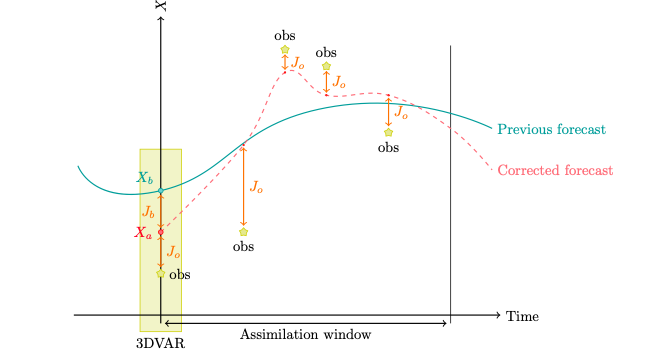
\includegraphics[width=0.8\textwidth]{"images/schema_3D_Var.png"}
	\end{center}
\subsubsection{From 3DVar to BLUE}
\noindent We have are 3D-Var cost function:
$$J(x)=\frac{1}{2}\|x-x^b\|_B^2+\frac{1}{2}\|H(x)-y\|_{R}^2 $$
 Let us minimize J and compute the variation of $J(x)$ with respect to
a variation of $x$ :
$$\begin{aligned}
\delta J(x)=&\frac{1}{2}(\delta x)^TB^{-1}(x-x^b) \\
&+\frac{1}{2}(x-x^b)^TB^{-1}\delta x \\ &+\frac{1}{2}(-H(\delta x))^TR^{-1}(y-H(x)) \\
&+\frac{1}{2}(x^b-H(x))R^{-1}(-H(\delta x)) \\
=&(\delta x)^TB^{-1}(x-x^b)-(\delta x)^TH^TR^{-1}(y-H(x)) \\
=&(\delta x)^T \nabla J
\end{aligned}$$
The extremum condition is 
$$\nabla J=B^{-1}(x^*-x^b)-H^TR^{-1}(y-Hx^*)=0$$
so we will have:
$$x^*=x^b+(B^{-1}+H^TR^{-1}H)^{-1}H^TR^{-1}(y-Hx^b)$$
Grave to Sherman-Morrison-Woodbury identity,
$$K^*=(B^{-1}+H^TR^{-1}H)^{-1}H^TR^{-1}=BH^T(R+HBH^T)^{-1}$$
Therefore, we have that our solution $x$ of the minimization problem coincides with the BLUE optimal analysis $x^a$
\subsection{Ensemble Kalman Filter}
\noindent We have seen so far two methods to do data assimilation, these methods are valid only for linear systems, but the Lorenz system is non-linear, that's why we will introduce the Ensemble Kalman Filter method which works well for non-linear systems. The ENKF method consists in using the Kalman filter method in high dimension and replace P by a set of states $x_1,x_2,..,x_{m}$. So we can approximate the moments of the error by the moments of the sample.
The we have:
$$x_i^a=x_i^f+K[y-h(x_i^f)]$$
We can also define the Kalman gains: 
$$K=P^f H^T(HP^f H^T+R)^{-1}$$
To begin with we can estimate the
forecast error covariance matrix as:
$$P^f=\frac{1}{m-1}\sum_{i=1}^{m}(x_i^f-\bar{x}^f)(x_i^f-\bar{x}^f)^T~~with~~\bar{x}^f=\frac{1}{m}\sum_{i=1}^{m}x_i^f $$ 
We can factorized the forecast error covariance matrix by:
$$P^f=X_f X_f^T$$
where $X_f$ is an $n \times m$ matrix whose columns are the normalized anomalies or normalized perturbations,
$$[X_f]_i=\frac{x_i^f-\bar{x}^f}{\sqrt{m-1}}$$
In addition, we have:
$$
\bar{x}^a=\frac{1}{m}\sum_{i=1}^mx_i^a~~,~~~~[X_a]_i=\frac{x_i^a-\bar{x}^a}{\sqrt{m-1}} $$	

	\newpage

	\section{Conclusion}
	\noindent To conclude all this and to summarize everything, we had as main goal to implement a parallel time resolution method for the Lorenz system, and to realize the data assimilation using the EnKF method. But to achieve these goals we had to understand the Lorenz system and try to implement several numerical resolutions to find a solution. Part explanation para-real. And finally for the data assimilation part we had to understand the principles of methods such as the Kalman filter and 3DVAR, it was also important to understand the link between these two methods in order to understand the method to use in the case where the differential equation system is nonlinear and to implement the method using EnKF with FilterPy. We noticed that during the data assimilation the covariance matrices associated with the error of our states had a very large impact on the analyses. Changing one of these parameters or reversing the covariance matrix associated with the error of the observations with the one associated with the model could seriously change our final analysis. For the future it would be interesting to explain the phenomenon seen in the part (cf. \ref{assimilation}), to understand why when we give a little more accuracy to the observation we observe that the curve of our states after data assimilation sticks much more to the observations.	
	
	\newpage	
	\bibliographystyle{plain}
	\bibliography{biblio}
	
\end{document}